\begin{filecontents*}{example.eps}
%!PS-Adobe-3.0 EPSF-3.0
%%BoundingBox: 19 19 221 221
%%CreationDate: Mon Sep 29 1997
%%Creator: programmed by hand (JK)
%%EndComments
gsave
newpath
  20 20 moveto
  20 220 lineto
  220 220 lineto
  220 20 lineto
closepath
2 setlinewidth
gsave
  .4 setgray fill
grestore
stroke
grestore
\end{filecontents*}
%\documentclass{svjour3}                     % onecolumn (standard format)
\RequirePackage{fix-cm}
%
%\documentclass{svjour3}                     % onecolumn (standard format)
%\documentclass[smallcondensed]{svjour3}     % onecolumn (ditto)
%\documentclass[smallextended]{svjour3}       % onecolumn (second format)
\documentclass[twocolumn]{svjour3}          % twocolumn
%
\smartqed  % flush right qed marks, e.g. at end of proof
%
\usepackage{appendix}
\usepackage{amsmath}
\usepackage{graphicx}
\usepackage[switch]{lineno}
\usepackage{array}
\usepackage{longtable}
\usepackage{natbib}
\usepackage{hyphenat}
\bibliographystyle{ieeetr}
\setcitestyle{square}
\setcitestyle{citesep={,}}


\linenumbers

\newcommand*\patchAmsMathEnvironmentForLineno[1]{%
\expandafter\let\csname old#1\expandafter\endcsname\csname #1\endcsname
\expandafter\let\csname oldend#1\expandafter\endcsname\csname end#1\endcsname
\renewenvironment{#1}%
{\linenomath\csname old#1\endcsname}%
{\csname oldend#1\endcsname\endlinenomath}}% 
\newcommand*\patchBothAmsMathEnvironmentsForLineno[1]{%
\patchAmsMathEnvironmentForLineno{#1}%
\patchAmsMathEnvironmentForLineno{#1*}}%
\AtBeginDocument{%
\patchBothAmsMathEnvironmentsForLineno{equation}%
\patchBothAmsMathEnvironmentsForLineno{align}%
\patchBothAmsMathEnvironmentsForLineno{flalign}%
\patchBothAmsMathEnvironmentsForLineno{alignat}%
\patchBothAmsMathEnvironmentsForLineno{gather}%
\patchBothAmsMathEnvironmentsForLineno{multline}%
}


%\documentclass[catalysts,article,submit,moreauthors,pdftex,10pt,a4paper]{mdpi} 
\usepackage{todonotes}
\usepackage{comment}
\usepackage{graphicx}
%--------------------
% Class Options:
%--------------------
% journal
%----------
% Choose between the following MDPI journals:
% actuators, admsci, aerospace, agriculture, agronomy, algorithms, animals, antibiotics, antibodies, antioxidants, applsci, arts, atmosphere, atoms, axioms, batteries, behavsci, beverages, bioengineering, biology, biomedicines, biomimetics, biomolecules, biosensors, brainsci, buildings, carbon, cancers, catalysts, cells, challenges, chemosensors, children, chromatography, climate, coatings, computation, computers, condensedmatter, cosmetics, cryptography, crystals, data, dentistry, designs, diagnostics, diseases, diversity, econometrics, economies, education, electronics, energies, entropy, environments, epigenomes, fermentation, fibers, fishes, fluids, foods, forests, futureinternet, galaxies, games, gels, genealogy, genes, geosciences, geriatrics, healthcare, horticulturae, humanities, hydrology, informatics, information, infrastructures, inorganics, insects, instruments, ijerph, ijfs, ijms, ijgi, inventions, jcdd, jcm, jdb, jfb, jfmk, jimaging, jof, jintelligence, jlpea, jmse, jpm, jrfm, jsan, land, languages, laws, life, literature, lubricants, machines, magnetochemistry, marinedrugs, materials, mathematics, mca, mti, medsci, medicines, membranes, metabolites, metals, microarrays, micromachines, microorganisms, minerals, molbank, molecules, mps, nanomaterials, ncrna, neonatalscreening, nutrients, particles, pathogens, pharmaceuticals, pharmaceutics, pharmacy, philosophies, photonics, plants, polymers, processes, proteomes, publications, recycling, religions, remotesensing, resources, risks, robotics, safety, sensors, separations, sexes, sinusitis, socsci, societies, soils, sports, standards, sustainability, symmetry, systems, technologies, toxics, toxins, universe, urbansci, vaccines, vetsci, viruses, water
%---------
% article
%---------
% The default type of manuscript is article, but can be replaced by: 
% addendum, article, book, bookreview, briefreport, casereport, changes, comment, commentary, communication, conceptpaper, correction, conferencereport, expressionofconcern, meetingreport, creative, datadescriptor, discussion, editorial, essay, erratum, hypothesis, interestingimage, letter, newbookreceived, opinion, obituary, projectreport, reply, retraction, review, sciprints, shortnote, supfile, technicalnote
% supfile = supplementary materials
%----------
% submit
%----------
% The class option "submit" will be changed to "accept" by the Editorial Office when the paper is accepted. This will only make changes to the frontpage (e.g. the logo of the journal will get visible), the headings, and the copyright information. Also, line numbering will be removed. Journal info and pagination for accepted papers will also be assigned by the Editorial Office.
%------------------
% moreauthors
%------------------
% If there is only one author the class option oneauthor should be used. Otherwise use the class option moreauthors.
%---------
% pdftex
%---------
% The option pdftex is for use with pdfLaTeX. If eps figure are used, remove the option pdftex and use LaTeX and dvi2pdf.

%=================================================================

%------------------------------------------------------------------
% The following line should be uncommented if the LaTeX file is uploaded to arXiv.org
%\pdfoutput=1

%=================================================================
% Add packages and commands here. The following packages are loaded in our class file: fontenc, calc, indentfirst, fancyhdr, graphicx, lastpage, ifthen, lineno, float, amsmath, setspace, enumitem, mathpazo, booktabs, titlesec, etoolbox, amsthm, hyphenat, natbib, hyperref, footmisc, geometry, caption, url, mdframed

%=================================================================
%% Please use the following mathematics environments:

%% For proofs, please use the proof environment (the amsthm package is loaded by the MDPI class).
\makeatletter
%\def\@biblabel#1{}
%\renewenvironment{thebibliography}[1]
%     {\section*{\refname}%
%      \@mkboth{\MakeUppercase\refname}{\MakeUppercase\refname}%
%      \list{\@biblabel{\@arabic\c@enumiv}}%
%           {\settowidth\labelwidth{\@biblabel#1{}}%
%            \leftmargin\labelwidth
%            \advance\leftmargin16pt
%            \advance\leftmargin\labelsep
%            \setlength\itemindent{-16pt}
%            \@openbib@code
%            \usecounter{enumiv}%
%            \let\p@enumiv\@empty
%            \renewcommand\theenumiv{\@arabic\c@enumiv}}%
%      \sloppy
%      \clubpenalty4000
%      \@clubpenalty \clubpenalty
%      \widowpenalty4000%
%      \sfcode`\.\@m}
%     {\def\@noitemerr
%       {\@latex@warning{Empty `thebibliography' environment}}%
%      \endlist}
%\renewcommand\newblock{\hskip .11em\@plus.33em\@minus.07em}
\makeatother

\makeatletter
%\renewcommand{\@biblabel}[1]{{}\hfill}
\makeatother
%=================================================================
% Full title of the paper (Capitalized)
\title{Transition-Metal Dopants in TiO$_2$ for Photocatalytic Nitrogen Fixation}

% Authors, for the paper (add full first names)

\author{Benjamin M. Comer$^{1 \dagger}$, Max H. Lenk$^{2}^{\dagger}$, Aradhya P. Rajanala$^{3}$, Emma L. Flynn$^{4}$, Andrew J. Medford$^{1}$*}
% Authors, for metadata in PDF

% Affiliations / Addresses (Add [1] after \address if there is only one affiliation.)
%\address{
%$^{1}$ \quad School of Chemical and Biomolecular Engineering, Georgia Institute of Technology\\
%$^{2}$ \quad School of Materials Science and Engineering, Georgia Institute of Technology\\
%$^{3}$ \quad School of Physics, Georgia Institute of Technology\\
%$^{4}$ \quad School of Computer Science, Georgia Institute of Technology\\
%}

% Contact information of the corresponding author
%\corres{Correspondence: ajm@gatech.edu}

% Current address and/or shared authorship
%\firstnote{Current address: Affiliation 3} 
%\firstnote{These authors contributed equally to this work.}

\institute{
$^{1}$ School of Chemical and Biomolecular Engineering, Georgia Institute of Technology\\
$^{2}$ School of Materials Science and Engineering, Georgia Institute of Technology\\
$^{3}$ School of Physics, Georgia Institute of Technology\\
$^{4}$ School of Computer Science, Georgia Institute of Technology\\
$\dagger$ These authors contributed equally to this work. \\
* Correspondence \email{andrew.medford@chbe.gatech.edu}\\
  311 Ferst Drive NW, Atlanta, Georgia 30318 \\
  Tel.:+1 (404) 385-5531\\
           %  \\
%             \emph{Present address:} of F. Author  %  if needed
}
\authorrunning{B. Comer et. al.}
% Simple summary
%\simplesumm{}

% Abstract (Do not use inserted blank lines, i.e. \\) 


% Keywords
%\keyword{ammonia synthesis; single atom catalysis; \textit{d}-band model; density functional theory}

% The fields PACS, MSC, and JEL may be left empty or commented out if not applicable
%\PACS{J0101}
%\MSC{}
%\JEL{}

% If this is an expanded version of a conference paper, please cite it here: enter the full citation of your conference paper, and add $^\S$ in the end of the title of this article.
%\conference{}

%%%%%%%%%%%%%%%%%%%%%%%%%%%%%%%%%%%%%%%%%%
% Only for the journal Data:

%\dataset{DOI number or link to the deposited data set in cases where the data set is published or set to be published separately. If the data set is submitted and will be published as a supplement to this paper in the journal Data, this field will be filled by the editors of the journal. In this case, please make sure to submit the data set as a supplement when entering your manuscript into our manuscript editorial system.}

%\datasetlicense{license under which the data set is made available (CC0, CC-BY, CC-BY-SA, CC-BY-NC, etc.)}

%%%%%%%%%%%%%%%%%%%%%%%%%%%%%%%%%%%%%%%%%%
\begin{document}


\maketitle
\begin{abstract}

%Developing novel, carbon-neutral methods of generating fixed nitrogen for chemicals and fertilizers is a vital step toward decarbonizing the global economy. TiO$_2$ has been observed to fix nitrogen at ambient pressure under illumination using only humidity and air. However, rates for this reaction remain low over a half-century after the discovery of the process. In this work, we investigate the use of surface metal dopants to promote surface reactions by altering the thermodynamics of intermediates on the rutile TiO$_2$ (110) surface. We screen all d-block transition metal dopants for stability and promotion of the reduction of nitrogen to ammonia. We find that the formation energy of surface metal dopant sites follows a trend described by the \textit{d}-band model, with sites becoming more stable from left to right on the periodic table. The binding energies of N$_2$, N$_2$H, and NH$_2$ all reach maximums on metal sites in the middle of the d-block. These energies trend with the cohesive energy as calculated by the Friedel model. The adsorption energies of intermediate species are correlated with each other and the \textit{d}-band center, suggesting that the \textit{d}-band model holds for single metal atoms doped into oxide surfaces. The catalytic activity of the metal-doped systems shows a volcano type relationship with the NH$_2$ binding energy as a descriptor. The metals predicted to be most active are Rh, Tc, and Co, but their activity is predicted to be comparable to that of Ti, indicating that metal-doped surface sites likely do not contribute significantly to photocatalytic nitrogen reduction.

%%%%%%%% catalysis letters requests an approximately 50 word abstract. I cut down the above text to be 60 words, as below:

In this work, we screen all d-block transition metal dopants for stability and promotion of the reduction of nitrogen to ammonia on TiO$_2$. The binding energies of N$_2$, N$_2$H, and NH$_2$ reach maximums on metal sites in the middle of the d-block. The activity of the metal-doped systems shows a volcano type relationship with the NH$_2$ energy as a descriptor.

\end{abstract}
\section{Introduction}
%%boilerplate Haber-Bosch intro
The fixation of atmospheric nitrogen has long been one of the prime challenges in chemistry and chemical engineering \cite{ritter_18, Schloegl_2003}. The Haber-Bosch process has been the route of choice for performing nitrogen fixation for the past century, permitting much of the population growth over that period \cite{Smil_1999}. However, this process has many significant drawbacks, including high CO$_2$ emissions and centralized production due to large capital requirements \cite{Comer_2019}. The Haber-Bosch process's considerable contribution to CO$_2$ emissions has been an increasingly pressing concern for the global community, as it is accountable for 340 million tonnes of CO$_2$---fully 2\% of the carbon emissions worldwide \cite{gross_12, Schiffer_2017}. For this reason, supplanting the Haber-Bosch process would represent a significant contribution to global efforts to curb climate change. Another drawback lies in the centralization of the Haber-Bosch process, which leads to high transportation costs and contributes to global economic inequality. \cite{Comer_2019} Due to the high pressures and pure feedstocks required, Haber-Bosch has significant economies of scale. Constructing a new plant requires significant capital and natural resources, as well as a critical mass of demand. Industrialized nations meet these criteria through a steady availability of capital and industrialized agricultural with a reliable demand for fertilizer. \cite{McArthur_2017} However, these barriers have prevented developing regions, such as Sub-Saharan Africa, from developing Haber-Bosch plants. The lack of local production results in high costs of fertilizers due to transportation, corresponding to reduced crop yields, which lowers demand and further increases prices. \cite{yuan_2014, IFDC_2012} This causes the fertilizer to be most expensive in regions where it is most needed.

Due to the various drawbacks of the Haber-Bosch process, researchers have sought alternative means of producing fixed nitrogen \cite{Comer_2019, McPherson_2019,WANG20181055, Kyriakou_2017}. These methods typically focus on optimizing catalyst structure under different conditions, but also extend to techniques such as genetically engineered crops using biological fixation. An example is chemical looping, a process in which nitrogen is hydrogenated by a metal hydride, released through oxidation of the metal, and the metal is subsequently rehydrogenated \cite{Michalsky_2015}. Chemical looping suffers from the high temperatures required for the metal rehydrogenation. Two catalysis focused strategies that have received significant recent interest are electrocatalysis \cite{McPherson_2019} and photocatalysis \cite{Medford_2017}. However, making either of these technologies viable presents a significant challenge. Electrochemical nitrogen fixation requires generating electricity and transporting electrons to the catalyst surface to perform the reaction \cite{Kyriakou_2017}. The need for both solar and electrocatalytic cells may limit the viability of electrochemical processes in the developing world \cite{Comer_2019}. An alternative route is photochemical nitrogen fixation, where the catalyst is placed in direct contact with sunlight and humidified air to produce fixed nitrogen. The photochemical route has the potential to operate with low capital investment and simpler infrastructure, making it promising for low-resource environments.

%review photocatalytic nitrogen fixation experiments, then a paragraph on metal/nonmetal doping
Photochemical nitrogen fixation has been known to the scientific community for decades, but inconsistent results and low rates have discouraged further study.\cite{Medford_2017} Photocatalytic nitrogen fixation was first hypothesized by N. Dhar, \cite{Dhar_1941} and the first well-controlled experiments were performed decades later when Schrauzer and Guth independently re-discovered the process \cite{Schrauzer_1977}. Schrauzer and Guth were able to establish the production of NH$_3$ in sterilized desert sands under illumination, \cite{Schrauzer_1977} including confirmation via isotopic labeling \cite{Schrauzer_1983}. Numerous independent experiments have been performed over the years and reported photochemical production of NH$_3$ over titania materials \cite{Bickley_1979,Augugliaro_1982,Soria_1991,Li_2018,Yuan_2013,Hirakawa_2017}, though legitimate skepticism has remained due to issues with contamination \cite{edwards1992opinion, Davies1995, davies1993reply}, interference,\cite{Gao_2018,Cui2018} and inconsistent results \cite{Medford_2017}. However, recent experiments utilizing ambient pressure X-ray Photoelectron Spectroscopy (AP-XPS) have observed reduced nitrogen compounds under only under illumination, providing direct experimental evidence that photo-induced nitrogen reduction occurs on titania surfaces, though the presence of carbon-based impurities was found to be a critical enabler of the process.\cite{Comer_2018b} %Indeed, it has proven critical to ensure great care is taken in NH$_3$ measurement methods, due to the low concentrations and interference of other species.\cite{Gao_2018,Cui2018}

%describe difference between photochemical and electrochemical systems

%discuss efficiency
Despite improved understanding of photocatalytic nitrogen fixation, the rates of reaction on titania-based catalysts remain relatively low ($\mu mol$ scale \cite{Hirakawa_2017}). The competition of NH$_3$ production with H$_2$ evolution is a key issue for electrocatalytic or photocatalytic nitrogen fixation, and has been dubbed the ``selectivity challenge''.\cite{Singh_2017} For this reason, high Faradic efficiency is also often sought in the electrochemical literature \cite{McPherson_2019}. The driver of this is the opportunity cost of using electricity for catalysis over other possible uses. For this reason, many electrochemical studies focus on low-overpotentials where the selectivity is generally highest, but the overall reaction rate is relatively low. In contrast, photo-excited electrons are difficult to harvest for alternate uses, and hence the overall solar-to-ammonia efficiency is the key metric for assessing photocatalytic ammonia production. Rates on the order of 0.001\% solar-to-ammonia efficiency have been reported for pure titania catalysts \cite{Hirakawa_2017}. This is substantially lower than the $\sim$20\% solar-to-hydrogen efficiency achieved by state-of-the-art catalytic systems for solar hydrogen production \cite{Nakamura_2015, Jia_2016}. However, it has been posited that a comparatively low solar efficiency of $\sim$0.1-1\% may be sufficient to enable solar fertilizer technology \cite{Comer_2019,Medford_2017}. With sufficiently low capital cost, this system could see use in areas that are far from fertilizer plants due to lowering of transportation costs. This indicates that strategies for enhancing the rate of photocatalytic ammonia production on titania catalysts may be a viable route for designing photocatalytic nitrogen fixation catalysts.

One route to increasing reaction rates is the the inclusion of transition\hyp{}metal dopants in TiO$_2$ \cite{Zaleska_2008}.  Transition\hyp{}metal dopants can increase rates via two distinct mechanisms: increasing the amount of photo-generated electrons that reach the surface by improving absorption and charge separation, or by altering the kinetics of the surface reaction.
%Doping metals within a semi-conductor can improve reaction rates by either altering the kinetics of the surface reaction or improving the material's photochemical properties of the material, such means as decreasing the band gap and tuning band alignment. 
Transition-metal doping has been previously explored to improve performance of TiO$_2$ photocatalysts \cite{Schneider_2014, Li_2007, Dozzi_2013}. In particular, early work on photocatalytic nitrogen fixation tested a variety of metal dopants, and it was reported that several noble metals \cite{Ranjit_1996} and iron in particular increase yields \cite{Schrauzer_1977,Schrauzer_1983, Augugliaro_1982,Soria_1991, Ranjit_1996,Ranjit_1997}. More recently, Hirakawa et al. found that depositing noble metals (Ru, Pt, Pd) onto an already prepared rutile (110) surface led to a decrease in reaction rates.\cite{Hirakawa_2017} This, along with detailed experimental and theoretical studies on the role of iron dopants ,\cite{Soria_1991, Comer_2018} suggests that the primary mechanism of these previously-reported dopants is enhanced charge separation. However, transition-metal dopants are also known to affect the surface properties in a range of other materials and reactions \cite{Khan_2018,Gu_2014, Ammal_2016, Gu_2017,Comer_2018, Garc_a_Mota_2011, Yao_2017}. In particular, the field of ``single-atom catalysis'' has revealed that isolated transition-metal sites supported on oxide materials can exhibit remarkable catalytic properties \cite{Liu_2016, Qiao_2011, O_Connor_2018}. However, relatively little effort has been focused on understanding how isolated transition-metal atom dopants affect the surface reactivity of oxides for conversion of nitrogen to ammonia \cite{Tao_2019, Liu_2019, Zhao_2019, Cheng_2019, Li_2017}.

%While much is known about the ability of dopant metals to change the bulk properties of a semiconducting material, however, photochemists rarely consider how doped metals at the surface could affect reaction kinetics. There is a sizable literature on the effects of metal sites in 2D materials\cite{Khan_2018}, and single atoms on oxide supports\cite{Liu_2016} and doped metal oxides \cite{Gu_2014, Ammal_2016 Gu_2017,Comer_2018, Garc_a_Mota_2011, Yao_2017}. This work focuses on doped metal oxide materials. 

%review theoretical work

%To expedite the process, avoiding a multitude of experimental tests on the domain of possible dopants, there have been attempts to predict catalytic activity computationally. Computational screening has been used profitably in several areas of catalysis including CO$_2$ reduction\cite{}, hydrogen evolution\cite{}, and oxygen reduction\cite{Norskov_004}. These theoretical studies screening materials for effectiveness in nitrogen fixation have confirmed its applicability as a predictive method.\cite{Hoskuldsson_2017} Theoretical results verify that the N$_2$ bond dissociation is the rate-limiting step. \cite{https://pubs.acs.org/doi/pdf/10.1021/jp056982h} Further endeavors focus on determining specific reaction pathways or finding more efficient ceramics, surfaces, and dopants.\cite{}
%describe challenges of ambient temperature N2 fixation

%The two largest challenges to fixing nitrogen under ambient conditions have been posited to be the kinetics of the first hydrogenation step and the desorption of NH$_3$ starting from NH$_2$.\cite{Hoskuldsson_2017,Singh_2017,Montoya_2015} These two challenges provide the basis of two design criteria for nitrogen fixation catalysts. N$_2$ is a molecules with no intrinsic dipole and a very strong N-N triple bond making reactions challenging at room temperature.\cite{Montoya_2015, Comer_2018}. This is the primary reason the first hydrogenation step is found to be rate limiting for low temperature nitrogen reduction.\cite{Montoya_2015, Singh_2017, Hoskuldsson_2017, Comer_2018} 
%The exceedingly high temperatures of the Haber-Bosch process (700K) allow it to follow a "dissociative" mechanism, whereby N$_2$ is dissociated on the catalyst surface into nitrogen adatoms immediately in the first step \cite{Ullmann_amm_2006, Hellman_2006}. Surmounting such a high energy barrier is not feasible at room temperature, requiring the reaction to follow an "associative" mechanism in which hydrogen atoms are attached successively to the nitrogen until the N-N bond can be broken.\cite{Montoya_2015} However, in cases where  NH$_x$ species tend to bind strongly to surfaces, making desorption of NH$_x$ species into the product NH$_3$ rate limiting. In the literature, the reaction from adsorbed NH$_2$* to fully desorbed NH$_3$ has been identified as rate limiting on catalysts with lower barrier for the first hydrogenation \cite{Hoskuldsson_2017}.

% review what we did in this publication then lead into results
In this work, we focus on the potential of isolated transition-metal atoms substituted into the rutile (110) titania surface as a potential route to improve the surface kinetics of the nitrogen reduction reaction. We screen The d-block transition metals substituted onto the (110) surface in two different configurations corresponding to formal oxidation states of 2+ and 4+. The 4+ slabs were generated by replacing the coordinatively unsaturated Ti with the studied metal. 2+ slabs were generated by substituting a 6 fold Ti with the substituent metal and adding an oxygen vacancy at the bridging oxygen site such (see Figure \ref{fig:ex_slab}). We analyze the trends present across the periodic table with for the dopant formation energy, N$_2$ adsorption energy, N$_2$H, and NH$_2$ adsorption energy. We also map out the thermodynamics of both associative and dissociative N$_2$ reduction pathways and use this to assess the most favorable reaction mechanism. Finally, we assess the expected improvement in reaction rates that is expected from forming metal dopant sites on the surface for photocatalytic N$_2$ reduction. The results illustrate that there are clear correlations in formation energy and surface reactivity with the \textit{d}-band center, resulting in a clear optimum in the rate-limiting potential for nitrogen reduction. However, the optimum dopants are not predicted to be significantly more active than pure TiO$_2$, suggesting that transition-metal doping is not a good strategy for tuning the reactivity for photocatalytic ammonia fixation on titania. Nonetheless, the strong trends observed indicate that the \textit{d}-band center is a good descriptor of reactivity for metal dopants on titania. This suggests that the \textit{d}-band model is a promising approach for selecting metal dopants in other oxide systems or designing single-atom catalysts supported on oxide materials.

\section{Results and Discussion}

Rutile TiO$_2$ (110) was chosen as a model surface based on experimental correlation between rutile content and reaction rates for photocatalytic nitrogen fixation\cite{Schrauzer_1977}. Additionally, there is a rich literature on the surface science of rutile (110) \cite{Diebold2003,Yates_1991,Lu1994,Walle2009}, and recent surface-science experiments and DFT calculations indicate that carbon substitution defects on the rutile (110) surface are active for photocatalytic nitrogen reduction \cite{Comer_2018b}. From this model surface, slabs containing metal dopants at the surface in the 2+ state were generated for each dopant metal. These 2+ sites were created by replacing the 6-fold titanium site with the substituent metal and removing a bridging oxygen (see Figure \ref{fig:ex_slab}.) 
%The 2+ oxidation state was chosen, as all transition metals are able to hold a 2+ oxidation state\cite{Greenwood_chemistry_text_book}, allowing trends to be seen across the periodic table. The stability of metal dopants in the 4+ oxidation states were also investigated, and found to be more stable in general(see Figure \ref{fig:d_band}). 
In total, all d-block transition-metals with the exception of Mn (24 total) were screened for their surface formation energy and activity for nitrogen reduction.  To study the reactivity of the generated surfaces, the binding energies of N$_2$H and NH$_3$ where investigated as they have been identified in the literature to be the rate limiting steps \cite{Hoskuldsson_2017, Montoya_2015, Comer_2018,}. Full details of the calculation methodology can be found in the methods section (Sec. \ref{sec:methods}).

%by mapping out the thermodynamics of all possible nitrogen reduction pathways on the surface. 

\begin{figure}
    \centering
    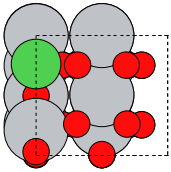
\includegraphics[width=0.5\linewidth]{Images/ex_2+_slab.png}
    \caption{An example of the screened 2+ slabs. The substituent metal has replaced a 6 fold Ti atom (seen in green) and a bridging oxygen vacancy has been formed to allow the metal to enter the 2+ oxidation state.}
    \label{fig:2+_ex_slab}
\end{figure}

\begin{figure}
    \centering
    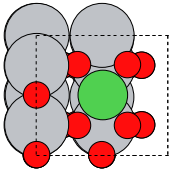
\includegraphics[width=0.5\linewidth]{Images/ex_4+_slab.png}
    \caption{An example of the screened 4+ slabs. The substituent metal has replaced a 5 fold Ti atom (seen in green) and a bridging oxygen vacancy has been formed to allow the metal to enter the 4+ oxidation state.}
    \label{fig:2+ex_slab}
\end{figure}

\subsection{Trends Across The Periodic Table}

%Studying the formation energy of 2+ metal substituted active sites and the binding energies of nitrogen species has revealed trends across the periodic table. The nature of these trends is based in electronic interactions between the metals' \textit{d}-band elections and the surface and adsorbates, as is commonly seen in catalysis \cite{Hammer_2000,Nilsson_2008, Greeley_2002}. However, full analysis of the electronic structures of these active sites is beyond the scope of this work, which focuses on the practical implications of the trends on catalytic systems.

\subsubsection{Active Site Formation Energies}

The stability of substituted metal surface sites has been examined with respect to the position of their \textit{d}-band center. In Figure \ref{fig:d_band} the formation energy of the studied active sites has been plotted against the location of the \textit{d}-band center of the corresponding transition metal. The formation energy of each metal substitute was calculated with respect to the pure metallic form. The \textit{d}-band centers are also calculated from the metallic bulk state rather than the single atom. Only metals where the \textit{d}-band center was previously reported in Ref. \citenum{Ruban_1997} are included in Figure \ref{fig:d_band}. The plot indicates there is a strong correlation between the \textit{d}-band center and formation energy of the metal substitution (R$^2$ = 0.89). We can rationalize the observed correlation in the context of the \textit{d}-band model of chemical bonding \cite{Nilsson_2008} summarized in Equation \ref{eq:d_band} below:

\begin{equation}
    %E_{coh} = \epsilon_d + \epsilon_s \\
    \Delta E_d = \int^{E_F} E(\rho'(E) - \rho(E))dE
    \label{eq:d_band}
\end{equation}

where $\Delta E_d$ is the binding energy associated with interaction with the \textit{d}-band, $E_F$ is the Fermi level energy, $\rho(E)$ is the \textit{d}-band density of states before adsorption, and $\rho(E)'$ is the density of states after adsorption. The interaction with s- states is assumed to be approximately constant for all metals, such that variations in binding energies are controlled primarily by the \textit{d}-band position. Interaction with the \textit{d}-band causes the orbitals of the adsorbate to separate into bonding and anti-bonding orbitals. As the \textit{d}-band center approaches the Fermi level the anti-bonding orbitals are increasingly filled, leading to a weaker bond.

In the case of formation energies, the system involves a metal atom interacting with an oxide surface rather than an adsorbate binding to the metal surface. However, it is hypothesized that the interaction between the \textit{d}-orbitals of the integrated metal atom interact with the p-band of the oxygen atoms in the surface in a manner similar to the metal surface interacting with an oxygen atom. This explanation is consistent with the observation that the interaction weakens from left to right on the periodic table. This implies that the metals most able to integrate into a surface are those with the most favorable interaction with oxygen. A similar relationship has been reported previously for doped rutile oxides \cite{Xu_2015} and oxide-supported single-atom catalysts \cite{O_Connor_2018}. Other reports suggest that the electronegativity of the substituted metal is the relevant descriptor predicting stability \cite{Garc_a_Mota_2011}. The electronegativity is also correlated with the formation energy (R$^2$=0.78 and 0.58 for 2+ and 4+ respectively, see Figure SXX), but not as strong as the correlation with the \textit{d}-band center of the metal (R$^2$=0.89 and 0.93, see Fig. \ref{fig:d_band}). The fact that both of these quantities correlate with the formation energy is not surprising, as the two quantities are both metrics of the propensity of the metal to accept electrons.


The only exceptions to this trend appear to be Ti, Zr, Hf, and Ag. The first three can be rationalized fairly easily, as all three lie in the same column of the periodic table which is the same column as the host metal, Ti. This affords approximately 1.5eV of improved stability relative to the trend. The improved stability of substituent metals within the group lines up with the chemical intuition since these elements have the same number of valence \textit{d} electrons. The final outlier, Ag, is more difficult to explain. When the elements are plotted with respect to their column on the periodic table (see Figure SXX), Ag is no longer an outlier, impling that the \textit{d}-band center of the corresponding transition metal is not a complete descriptor for the formation energies.

These data also have implications for the formation of surface metal clusters. Figure \ref{fig:d_band} indicates that the element's \textit{d}-band center controls the dopant metal's tendency to form surface-segregated sites or single-atom sites rather than integrate into the surface on TiO$_2$. This also has implications for the ability to synthesize metal-doped surfaces experimentally, showing that some elements (Y, Sc, Zr, Hf) favor integration into the surface structure rather than the formation of surface metal clusters (see table SXX). Conversely, noble metals such as Rh and Pt do not integrate into the surface favorably and will tend to form surface nano-clusters under thermodynamically equilibrated conditions. This result agrees with TEM measurements in the experimental literature, indicating that clusters of metals such as platinum and silver form on TiO$_2$ surfaces.\cite{Iliev_2006}\todo{find some more TEM work} % While this work only examines TiO$_2$, similar trends may exist in other metal oxide materials, warranting further investigation. %It should also be emphasized that this result refers to the formation of surface sites, not integrating into the bulk structure.

\begin{figure}
    \centering
    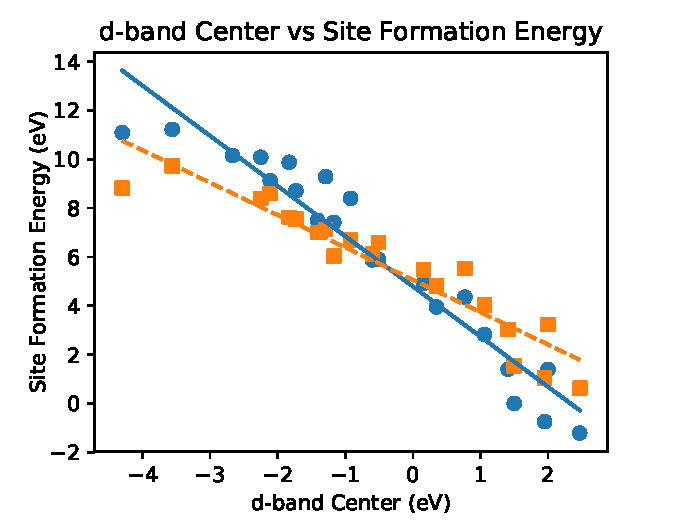
\includegraphics[width=0.9\linewidth]{Images/combined_d_band_vs_formation.pdf}
    \caption{Formation energy of surface sites with respect to their bulk metalic form vs the substituted metal's \textit{d}-band center as reported by Ruban et. al \cite{Ruban_1997}}
    \label{fig:d_band}
\end{figure}

%In Figure \ref{fig:2+_N2_react_stab} the formation energy of the surface vs binding energy of N$_2$ are shown. Both of these values are important to quantify, as an active site with an exceptionally high formation energy is unlikely to exist on the surface in any significant quantity. Because of the close relationship between the formation energy of 2+ metal substitutes and the valence number seen in Figure \ref{fig:valence} this plot may also be read as approximately showing the N$_2$ adsorption energy across the periodic row similar to Figure \ref{fig:2+_N2_period}. From a There are many sites that bind N$_2$ with an energy of $\approx$ -0.2eV, which represents a weak physorption interaction and is not sufficient to bind N$_2$ at room temperature. However, some metal sites bind N$_2$ in a manner related to the site's formation energy. The sites able to bind N$_2$ are all in the middle of the row as seen in Figure \ref{fig:2+_N2_period} This fact highlights the tradeoff between two trends: the adsorption of N$_2$ and surface formation energy. These metal sites yield a frontier of Pareto optimal surface sites for adsorbing N$_2$. This analysis indicates that the active site's relative instability is a necessary but not sufficient condition for increasing N$_2$ binding.

\subsubsection{Binding of Nitrogen Species}

The adsorption of the inert N$_2$ molecule is required for nitrogen fixation, and the first hydrogenation to N$_2$H is known to be the potential-limiting step on pure TiO$_2$ \cite{Comer_2018}. This suggests that the trends in N$_2$ and N$_2$H binding will provide an indication of a metal's ability to promote nitrogen reduction. The results for N$_2$ adsorption as a function of periodic table group are shown in Fig. \ref{fig:N2_rows}. The results deviate from the typical near-linear correlation that would be expected from the \textit{d}-band model, and instead show quadratic behavior with a maximum at Os near the middle of the \textit{d}-block. Similar results are found for N$_2$H adsorption (\ref{fig:N2H_rows}), though the magnitude of the adsorption energies vary, and the location of the maximum shifts slightly to Re. 

%Patterns in N$_2$ and N$_2$H can also be observed down the rows of the periodic table as seen in Figures \ref{fig:N2_rows}. It should be noted that the results for group 4 have not been included in the main text due to difficulties converging the electronic structures of the materials, making trends difficult to infer. The results for elements in group 4 that did converge may be seen in the supplementary information. The likely reason is the challenging magnetic states of several systems within this row. Figure \ref{fig:2+_N2_period} particularly shows the trend of increased N$_2$ binding down the periodic row, reaching a maximum in the center of the row and dropping more rapidly as the d-shell is filled. The results do not match the trends traditionally seen in the \textit{d}-band model\cite{Nilsson_2008} for transition metal binding energies; which would have the adsorption energy getting weaker moving left on the row. This is not surprising as the \textit{d}-band model was derived for transition metals, not doped metal oxides. In addition to the trend across the rows, the binding strength increases down the columns with Os having the strongest binding as well as being in the middle of the d-block and on the lowest tested row for N$_2$ binding. Finally it can be noted that the location of the maxima is not consistent between N$_2$ and NH$_2$, with the maxima for N$_2$ being two positions to the right of NH$_2$.


\begin{figure}
    
    \centering
    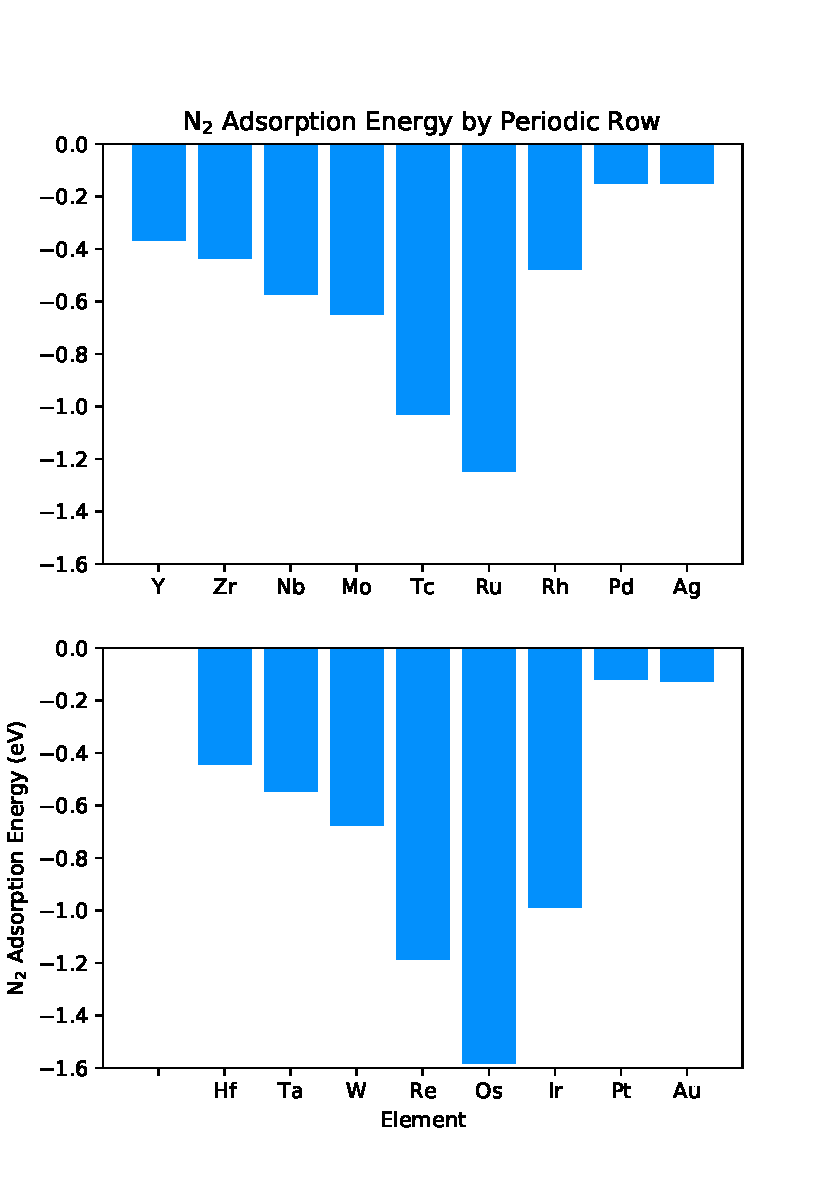
\includegraphics[width=0.5\textwidth]{Images/N2_adsorption_rows.pdf}
    \caption{The adsorption of N$_2$ on 2+ metal substituent sites for d block elements in rows 4 and 5.}
    \label{fig:N2_rows}
\end{figure}

\begin{figure}
    \centering
    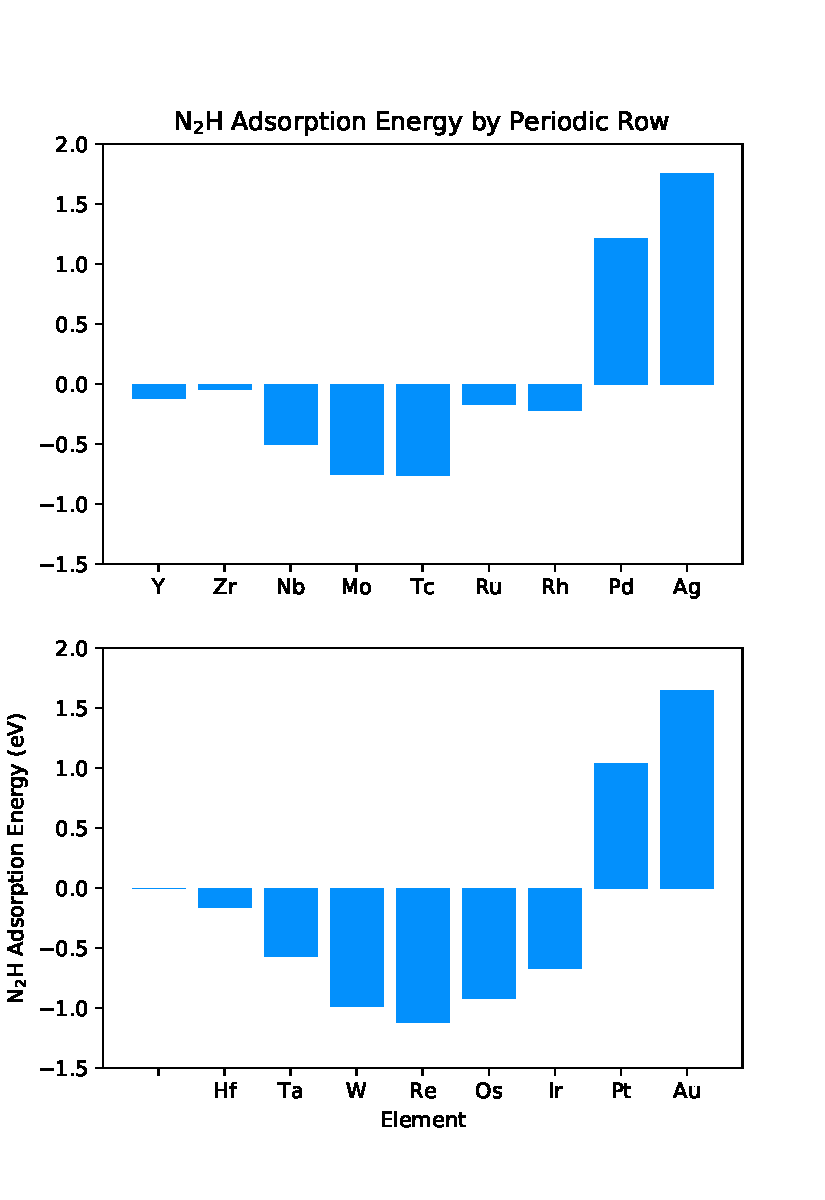
\includegraphics[width=0.5\textwidth]{Images/N2H_adsorption_rows.pdf}
    \caption{The adsorption of N$_2$H on 2+ metal substituent sites for d block elements in rows 4 and 5}
    \label{fig:N2H_rows}
\end{figure}

The trend in N$_2$ and N$_2$H binding observed deviates from the near-linear correlation that would be expected from the \textit{d}-band model. However, the binding energies of N$_2$H is linearly correlated with the \textit{d}-band contributions of the cohesive energies of the corresponding bulk systems (Fig. \ref{fig:N2H_cohesive}). The \textit{d}-band cohesive energy can be described by the the Friedel Model \cite{1969TPom}, which assumes a square shape for the \textit{d}-band, and is summarized in Equations \ref{eq:cohesive} and \ref{eq:d_band_cohesive}:


\begin{equation}
    E_{coh} = \epsilon_d + \epsilon_s
    \label{eq:cohesive}
\end{equation}
where $E_{coh}$ is the cohesive energy, $\epsilon_s$ is the \textit{s}-electron contribution to the cohesive energy (assumed to be constant for \textit{d}-block metals), and $\epsilon_d$ is the \textit{d}-electron contribution to the cohesive energy given by:

\begin{equation}
    \epsilon_d = \int^{E_F} (E_d-E)\rho(E)dE
    \label{eq:d_band_cohesive}
\end{equation}
where $E_F$ is the Fermi level energy, $E_d$ is the energy associated with broadening the \textit{d}-band, and $\rho(E)$ is the \textit{d}-band density of states of the material. 

The Friedel Model (Eq. \ref{eq:cohesive} and \ref{eq:d_band_cohesive}) and the \textit{d}-band model (Eq. \ref{eq:d_band}) both track the bonding and anti-bonding contributions of \textit{d} electrons. However, in the Friedel Model, the energy change is from fully isolated metal atoms to crystalline transition metals, and the \textit{d}-band is assumed to be a rectangular block. As a consequence, the bonding orbitals fill in the first half of the transition metal row, followed by the anti-bonding orbitals in the second half of the row. Thus, cohesive interactions strengthen in the first half of the row and weaken in the second half, creating a maxima when the \textit{d}-orbitals are half filled. The fact that N$_2$H binding follows a similar trend suggests that the $d$-band of the dopant metal atoms can be approximated by a rectangle, and that interactions with N$_2$H leads to a filling of bonding orbitals in the early transition metals, followed by filling of anti-bonding orbitals for the late transition metals. This is in contrast to the standard \textit{d}-band model, where only anti-bonding orbitals are created and filled due to the interaction between the \textit{d}-band and the molecular orbitals. 
%This suggests that the \textit{d}-band close to the fermi level is similarly rectangular.
%Additionally, the filling of the metal's \textit{d}-band for binding nitrogen species first fills up \textit{d}-bonding orbitals moving down the periodic row rather than merely anti-bonding orbitals as in the case for traditional \textit{d}-band model correlations. However, the lack of very tight correlation suggests that the assumptions the Friedel model makes about the \textit{d}-band do not hold for our system.

%when doped on a surface and the metal sublimating are similar.

%Thus, we hypothesize that these phenomena are governed by the same underlying physics. 

A similar trend is seen with N$_2$ adsorption in Figure \ref{fig:N2_cohesive}. however the correlation is much less predictive due to several elements displaying much stronger binding than would be expected by this model. The low $R^2$ value of this correlation implies that the system is more complicated than the case of N$_2$H. Thus, for the case of N$_2$ binding, increasing cohesive energy predicting increased binding is only a general trend. 

The existence of these trends shows the potential for tuning embedded metal sites to perform particular reactions. We based on our results and previous work \cite{Xu_2015,Garc_a_Mota_2011,Yao_2017} hypothesize that trends similar those found on TiO$_2$ apply to other metal oxides and crystal structures.

%In the  shows a reasonable correlation with the \textit{d}-band energy contribution to the cohesive energies of the bulk phases of the substituent metals as seen in Figure \ref{fig:N2H_cohesive}. This quantity may be obtained using equation \ref{eq:d_band_cohesive} below \cite{Gautier_1975}. The relationship implies that the \textit{d}-band contribution of the cohesive energy is related to the reactivity of the metal atom. Larger cohesive energy implies that the metal is more stabilized through bonding with itself, which can be thought of as the metal being more reactive. This trend does not match the one typically seen in the \textit{d}-band model, however the relationsh More reactive elements tend to lie in the center of the periodic row, due to their \textit{d}-band filling properties. The Friedel Model\cite{1969TPom} describes this in terms 

\begin{figure}
    \centering
    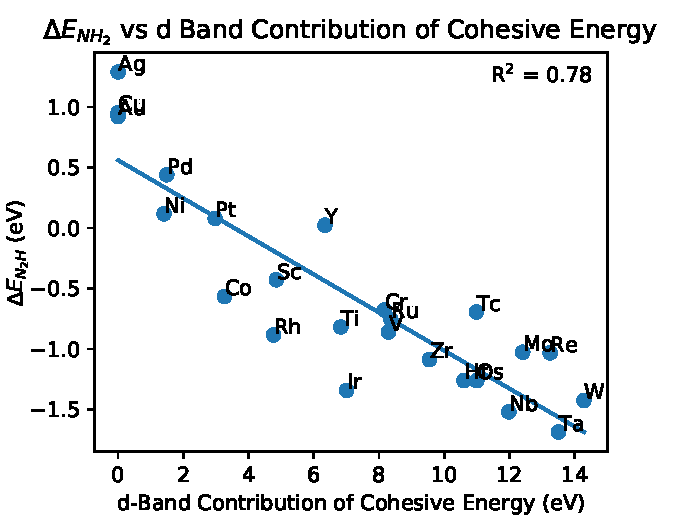
\includegraphics[width=0.4\textwidth]{Images/cohesive_eng_vs_N2H.pdf}
    
    \caption{The \textit{d}-band contribution to the cohesive energy of transition metals vs the N$_2$H binding energy of the metal substituted in the 2+ oxidation state in TiO$_2$. \textit{d}-band cohesive energy contributions obtained from Turchanin and Agraval\cite{Turchanin_2008}}
    \label{fig:N2H_cohesive}
\end{figure}

\begin{figure}
    \centering
    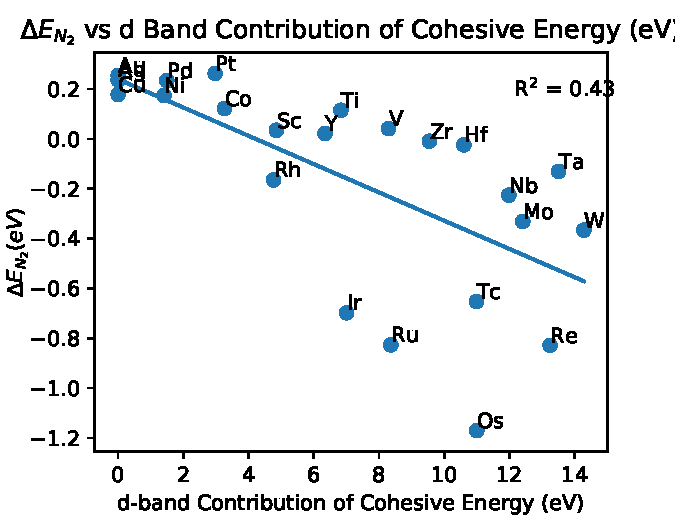
\includegraphics[width=0.4\textwidth]{Images/cohesive_eng_vs_N2.pdf}
    
    \caption{The \textit{d}-band contribution to the cohesive energy of transition metals vs the N$_2$ binding energy of the metal substituted in the 2+ oxidation state in TiO$_2$. \textit{d}-band cohesive energy contributions obtained from Turchanin and Agraval\cite{Turchanin_2008}}
    \label{fig:N2_cohesive}
\end{figure}

\begin{figure}
    \centering
    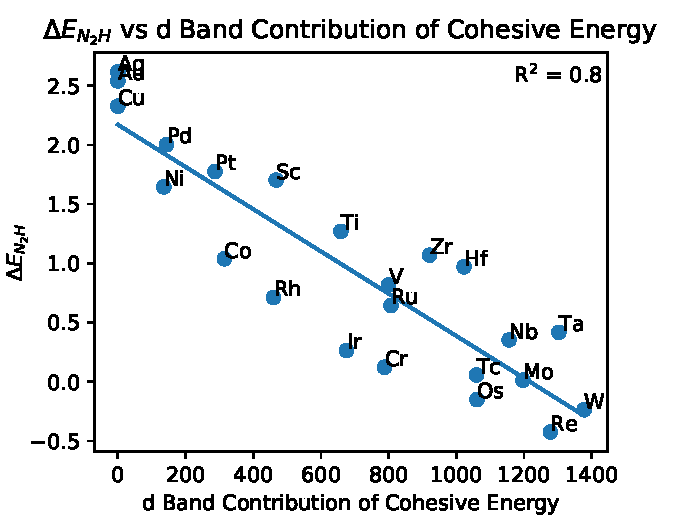
\includegraphics[width=0.4\textwidth]{Images/cohesive_eng_vs_NH2.pdf}
    
    \caption{The \textit{d}-band contribution to the cohesive energy of transition metals vs the N$_2$ binding energy of the metal substituted in the 2+ oxidation state in TiO$_2$. \textit{d}-band cohesive energy contributions obtained from Turchanin and Agraval\cite{Turchanin_2008}}
    \label{fig:N2_cohesive}
\end{figure}

%\begin{figure}
%    \centering
%    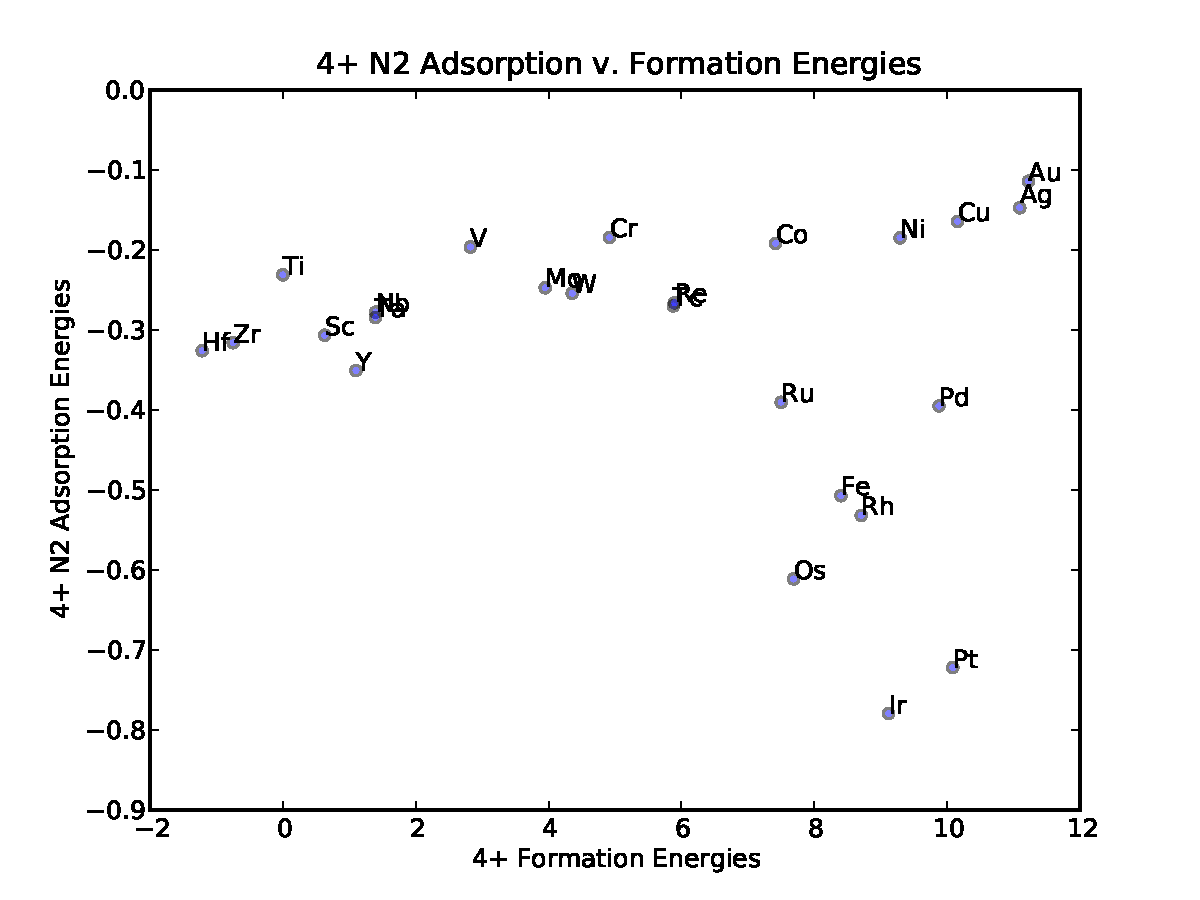
\includegraphics[width=0.8\linewidth]{Images/4+N2_Formation.pdf}
%    \caption{4+ Formation Energy versus N2 Adsorption Energy}
%    \label{fig:4+_N2_react_stab}
%\end{figure}
%\begin{figure}
%    \centering
%    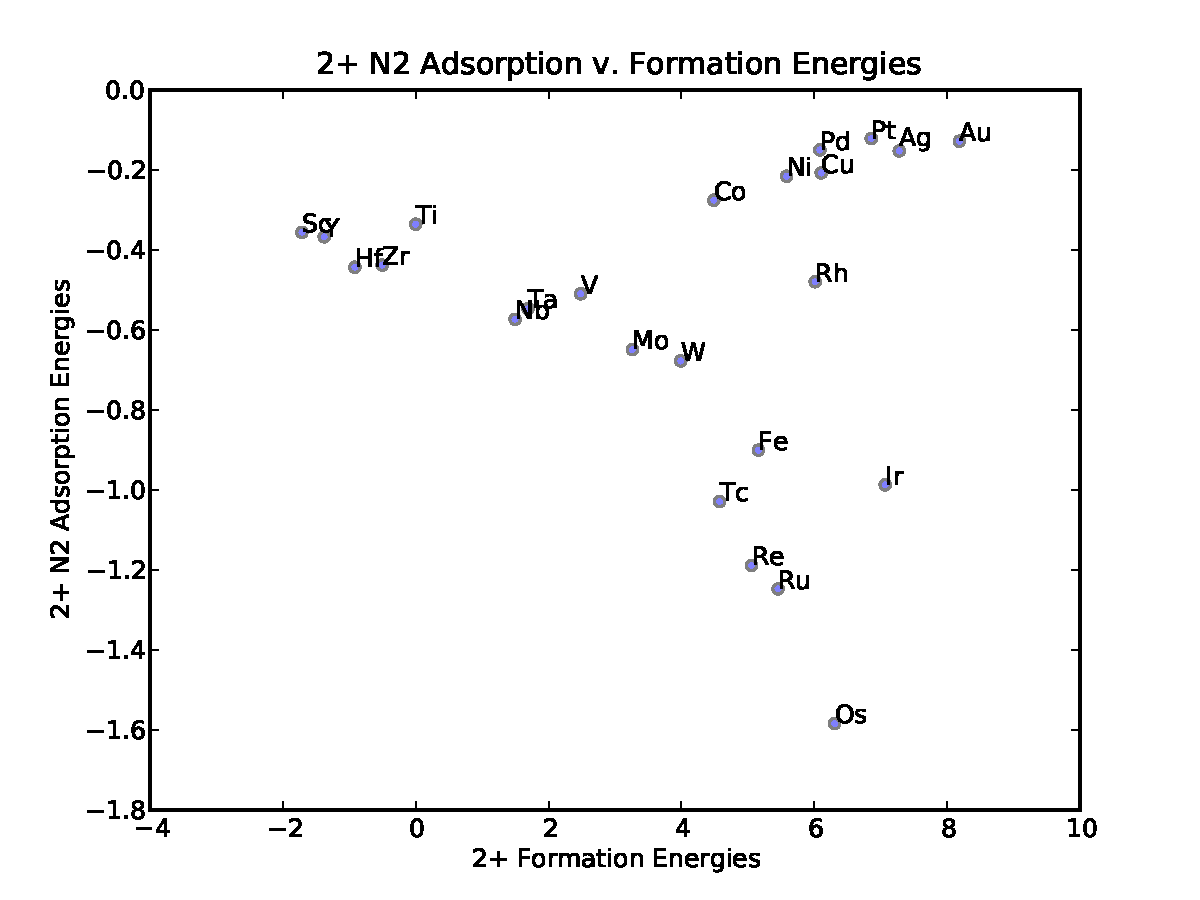
\includegraphics[width=0.8\linewidth]{Images/2+N2_Formation.pdf}
%    \caption{2+ Formation Energy versus N2 Adsorption Energy}
%    \label{fig:2+_N2_react_stab}
%\end{figure}
%The first hydrogenation step is commonly thought to be rate limiting, thus the third criterion is a reasonable N$_2$ $\rightarrow$ N$_2$H reaction energy. While some would also add NH$_2$ binding energy as a fourth criterion\cite{}, this was not evaluated. \todo{give a better reason why we didn't do this} However, these authors suggest that an N$_2$H binding energy of 0eV is the optimum for rutile oxides. 


%Based on this analysis we have identified X metals which show promise for photocatalytic nitrogen fixation. We completed reaction pathways for each of these reactions, the results can be seen in Figure \ref{}.\todo{discuss the results once we have the data}
%The adsorption of N$_2$ on dopant metals follows a clear trend across the rows of the periodic table as well as down the periodic columns (Figure \ref{}). The trend can be generally described by the \textit{d}-band model.\cite{Nilsson_2008}\todo{describe the \textit{d}-band model} 
%\textit{d}-band theory is an explanation of one factor involved in deciding the strength of the interaction between the molecule and the adsorbate. Because of the similarity of the s and p blocks of the transition metals, the most important interactions between the metal adsorbate and the molecule are with the \textit{d}-band. When the molecule and the metal adsorbate interact, they create both a bonding and antibonding state. The higher the filling of the antibonding state, the weaker the bonding is. This corresponds inversely with the height of the \textit{d}-band center; the higher the \textit{d}-band center, the less the antibonding state is filled. This theory predicts that near the center of the d block, the interactions will be stronger, corroborating our theory.




%\begin{figure}
%    \centering
%    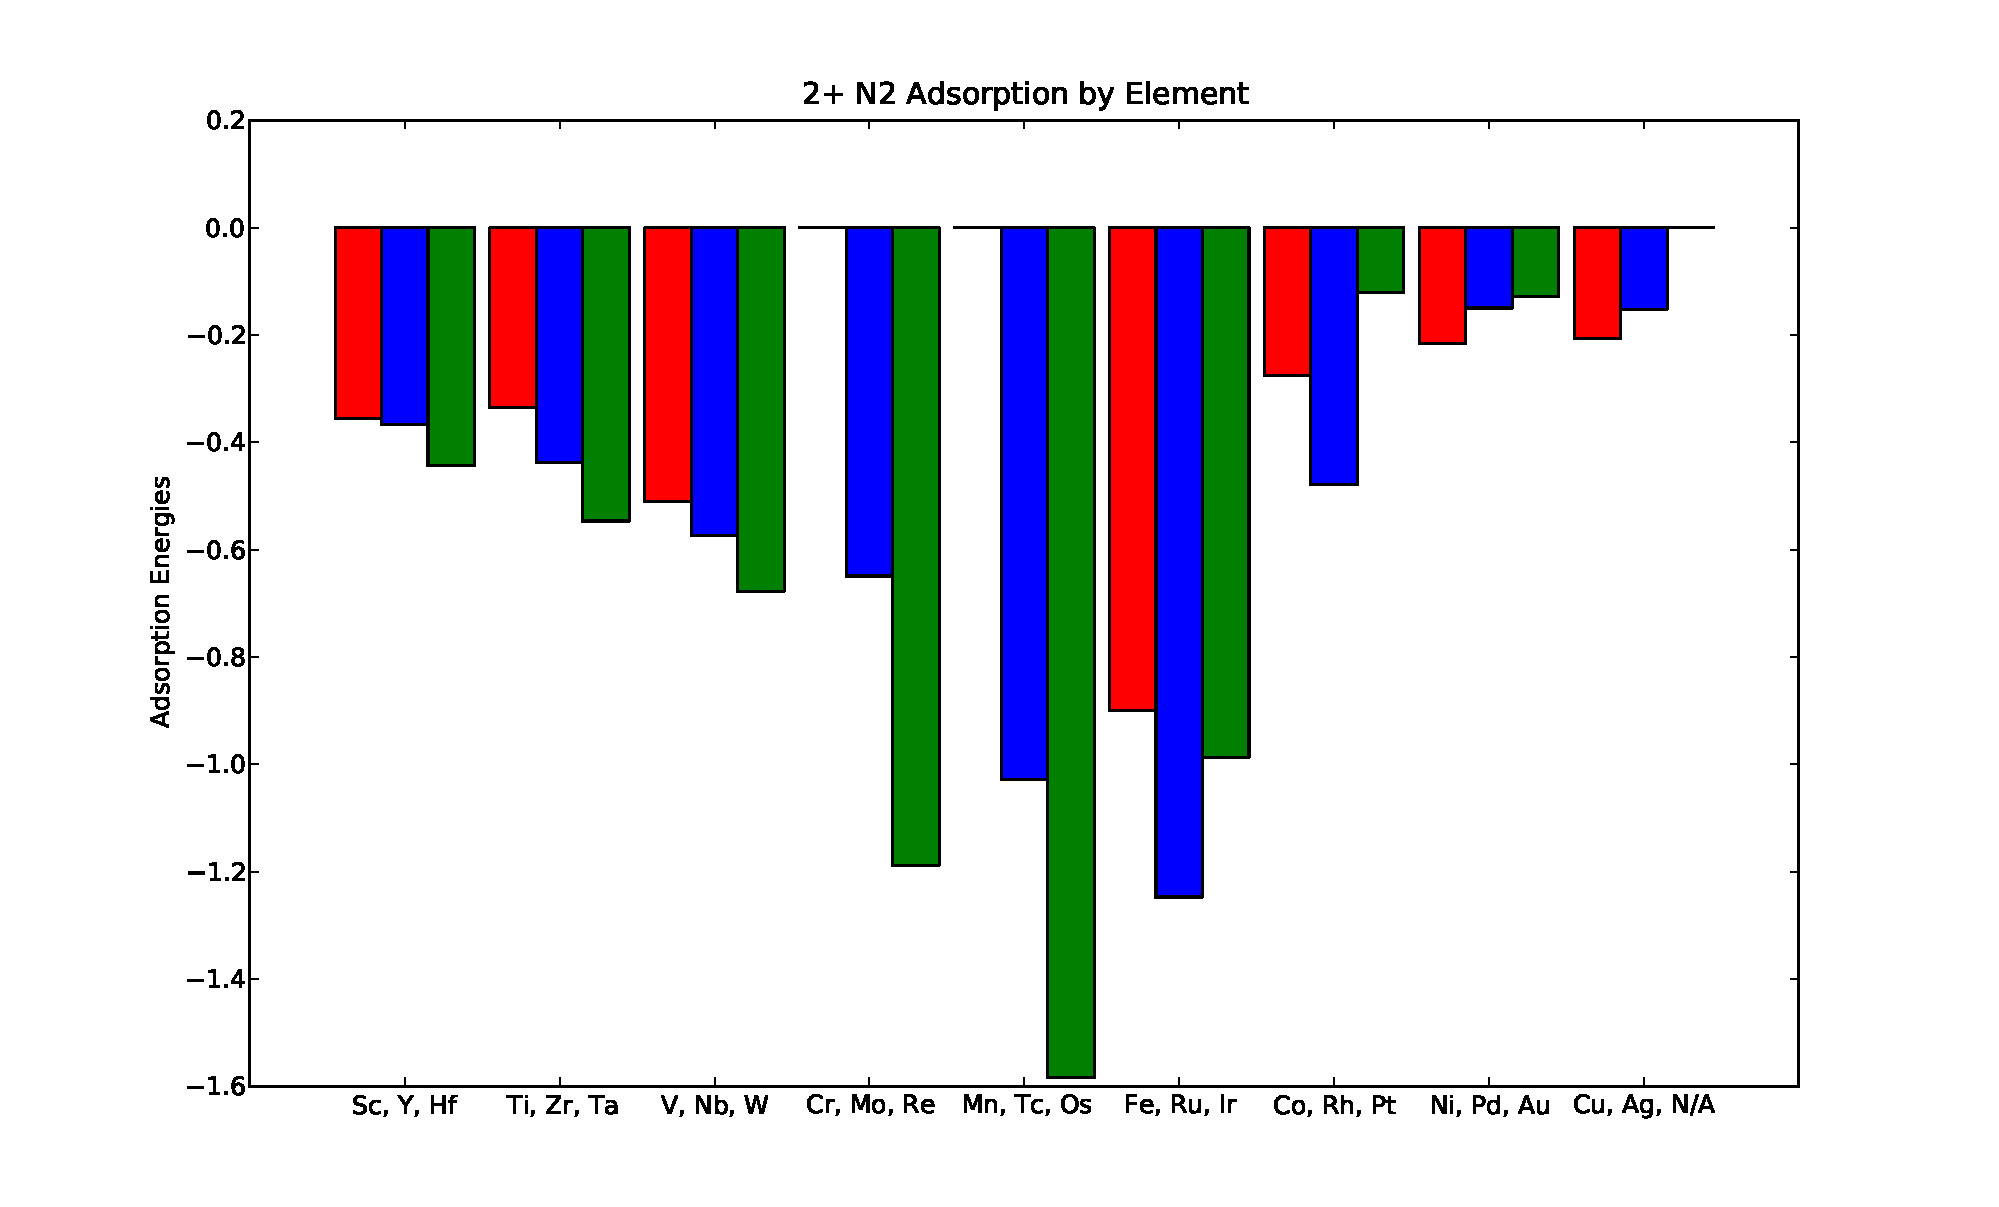
\includegraphics[width=0.8\linewidth]{Images/2+N2_by_element.pdf}
%    \caption{2+ N2 Adsorption Energy versus Element}
%    \label{fig:2+_N2_period}
%\end{figure}

%\begin{figure}
%    \centering
%    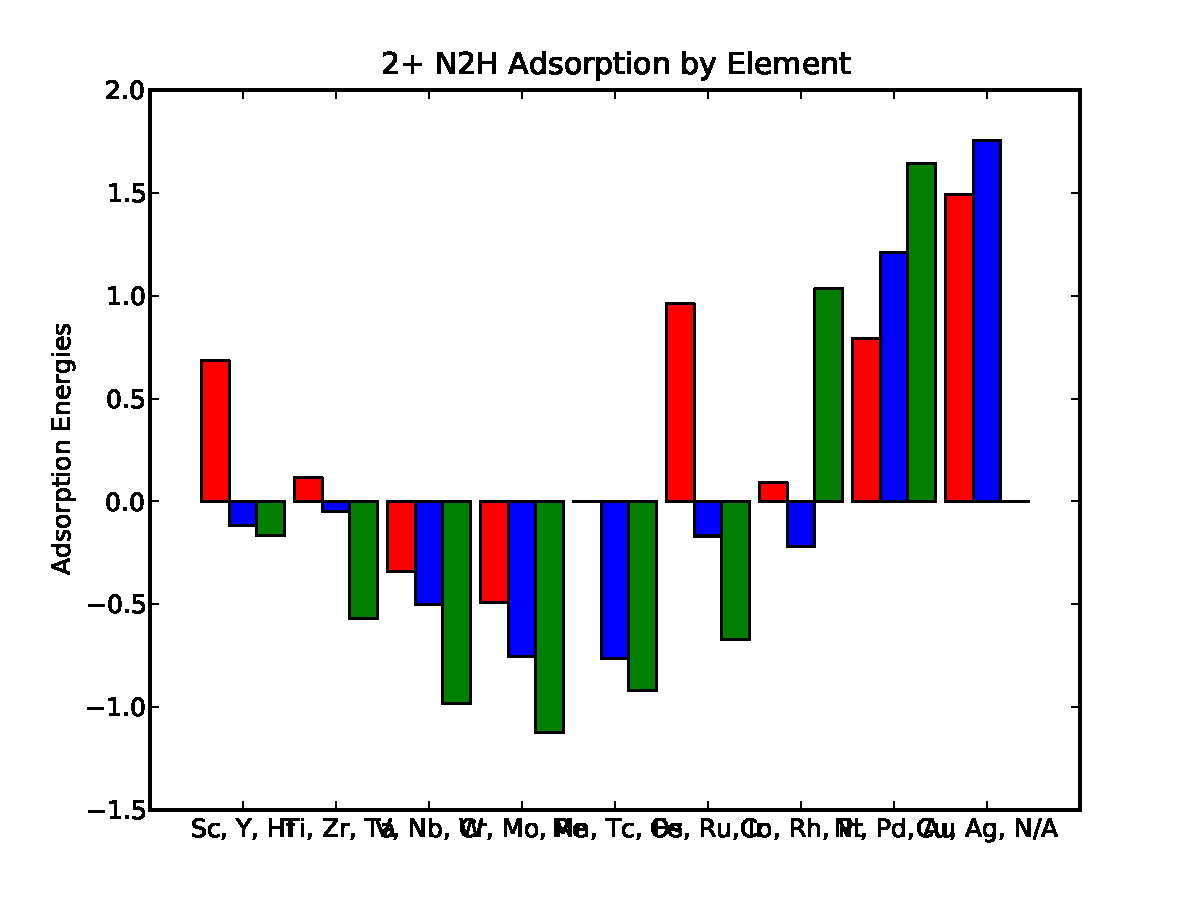
\includegraphics[width=0.8\linewidth]{Images/2+N2H_by_element.pdf}
%    \caption{2+ N2H Adsorption Energy versus Element}
%    \label{fig:2+_N2H_period}
%\end{figure}
%\begin{figure}
%    \centering
%    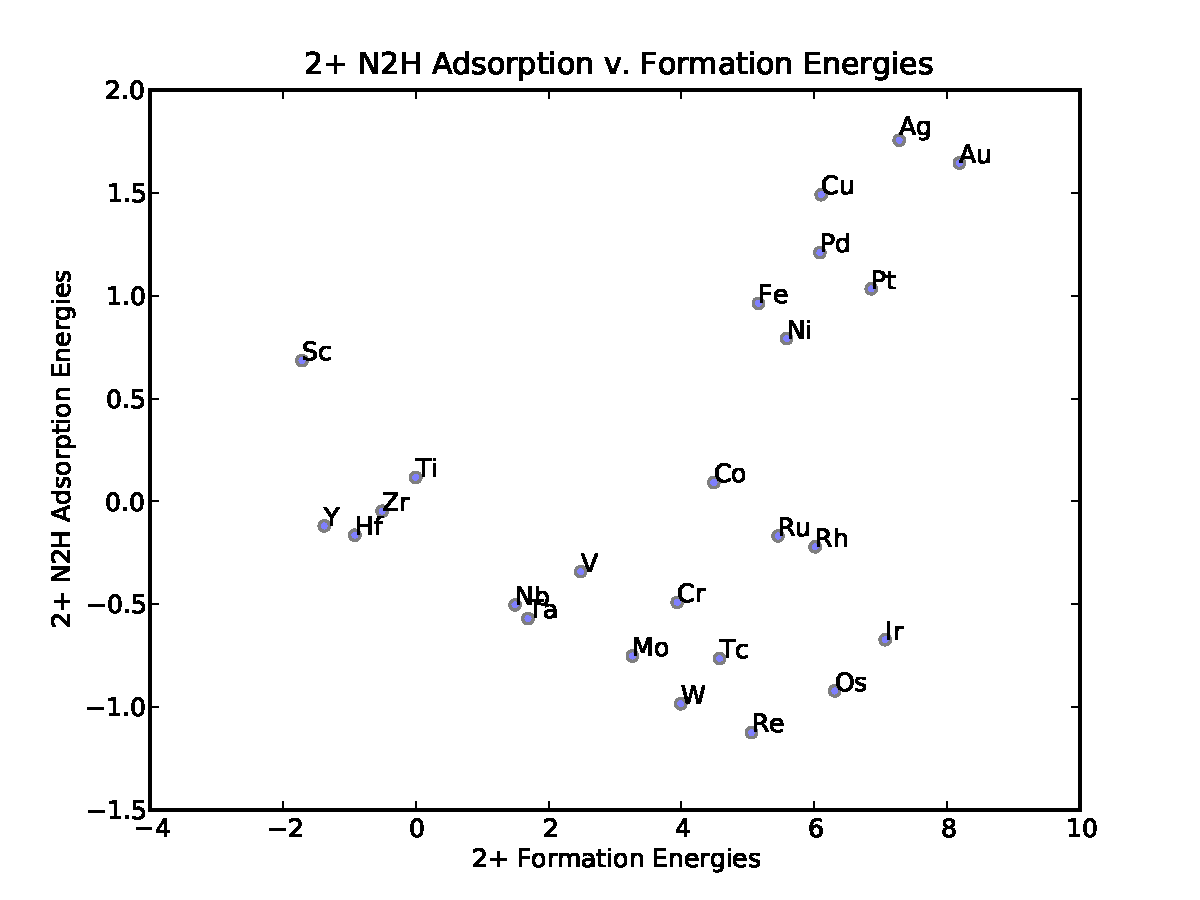
\includegraphics[width=0.8\linewidth]{Images/2+N2H_Formation.pdf}
%    \caption{2+ Formation Energy versus N2H Adsorption Energy}
%    \label{fig:2+_N2H_react_stab}
%\end{figure}
%\begin{figure}
%    \centering
%    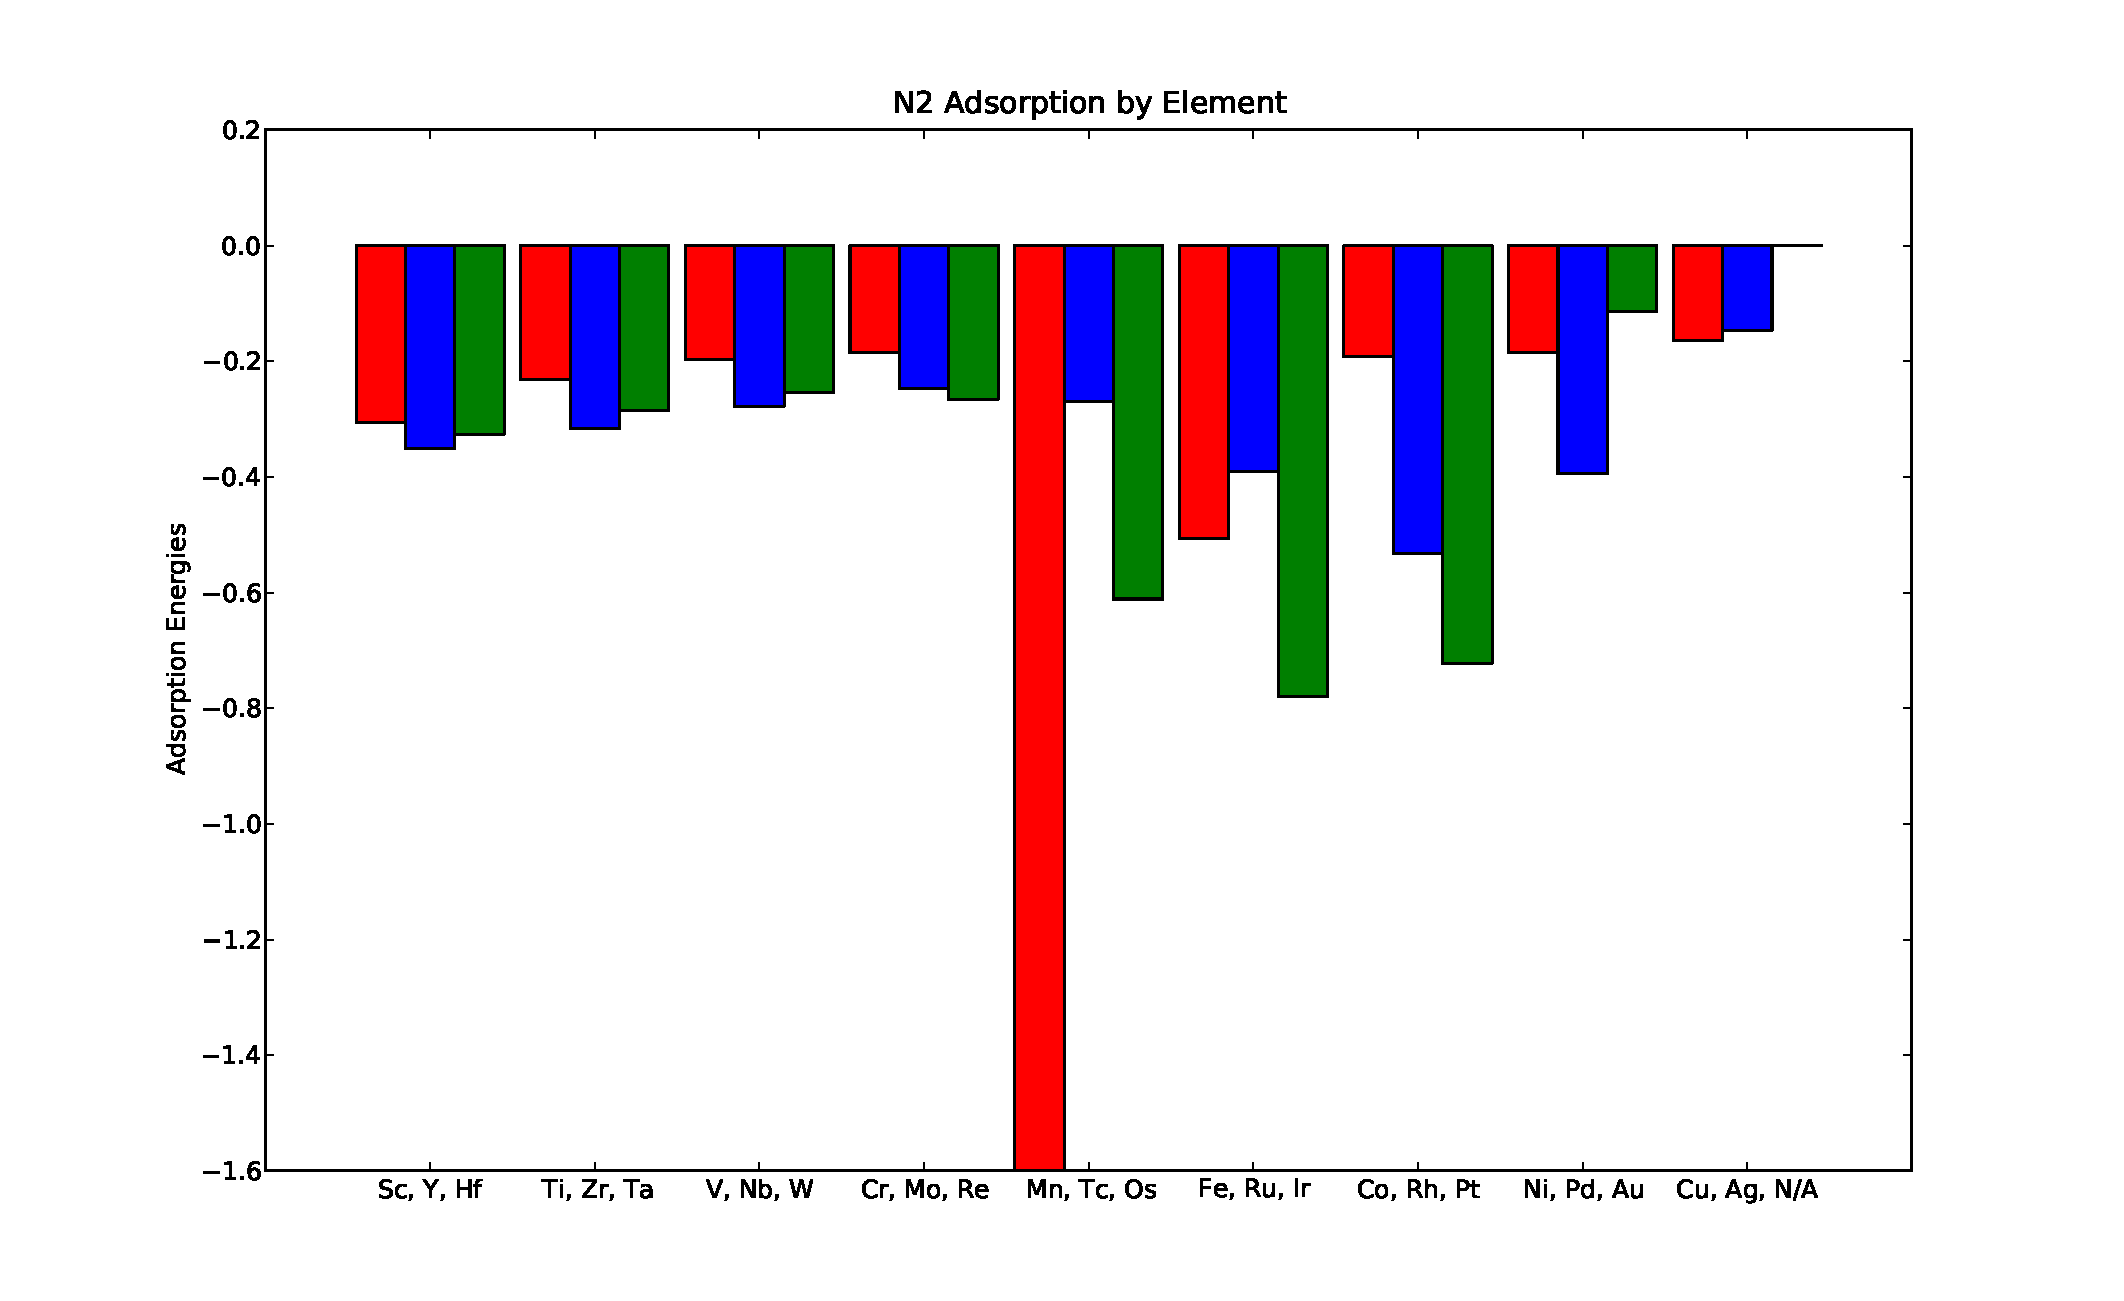
\includegraphics[width=0.8\linewidth]{Images/4+N2_by_element.pdf}
%    \caption{4+ N2 Adsorption Energy versus Element}
%    \label{fig:4+_N2_period}
%\end{figure}

%\begin{figure}
%    \centering
%    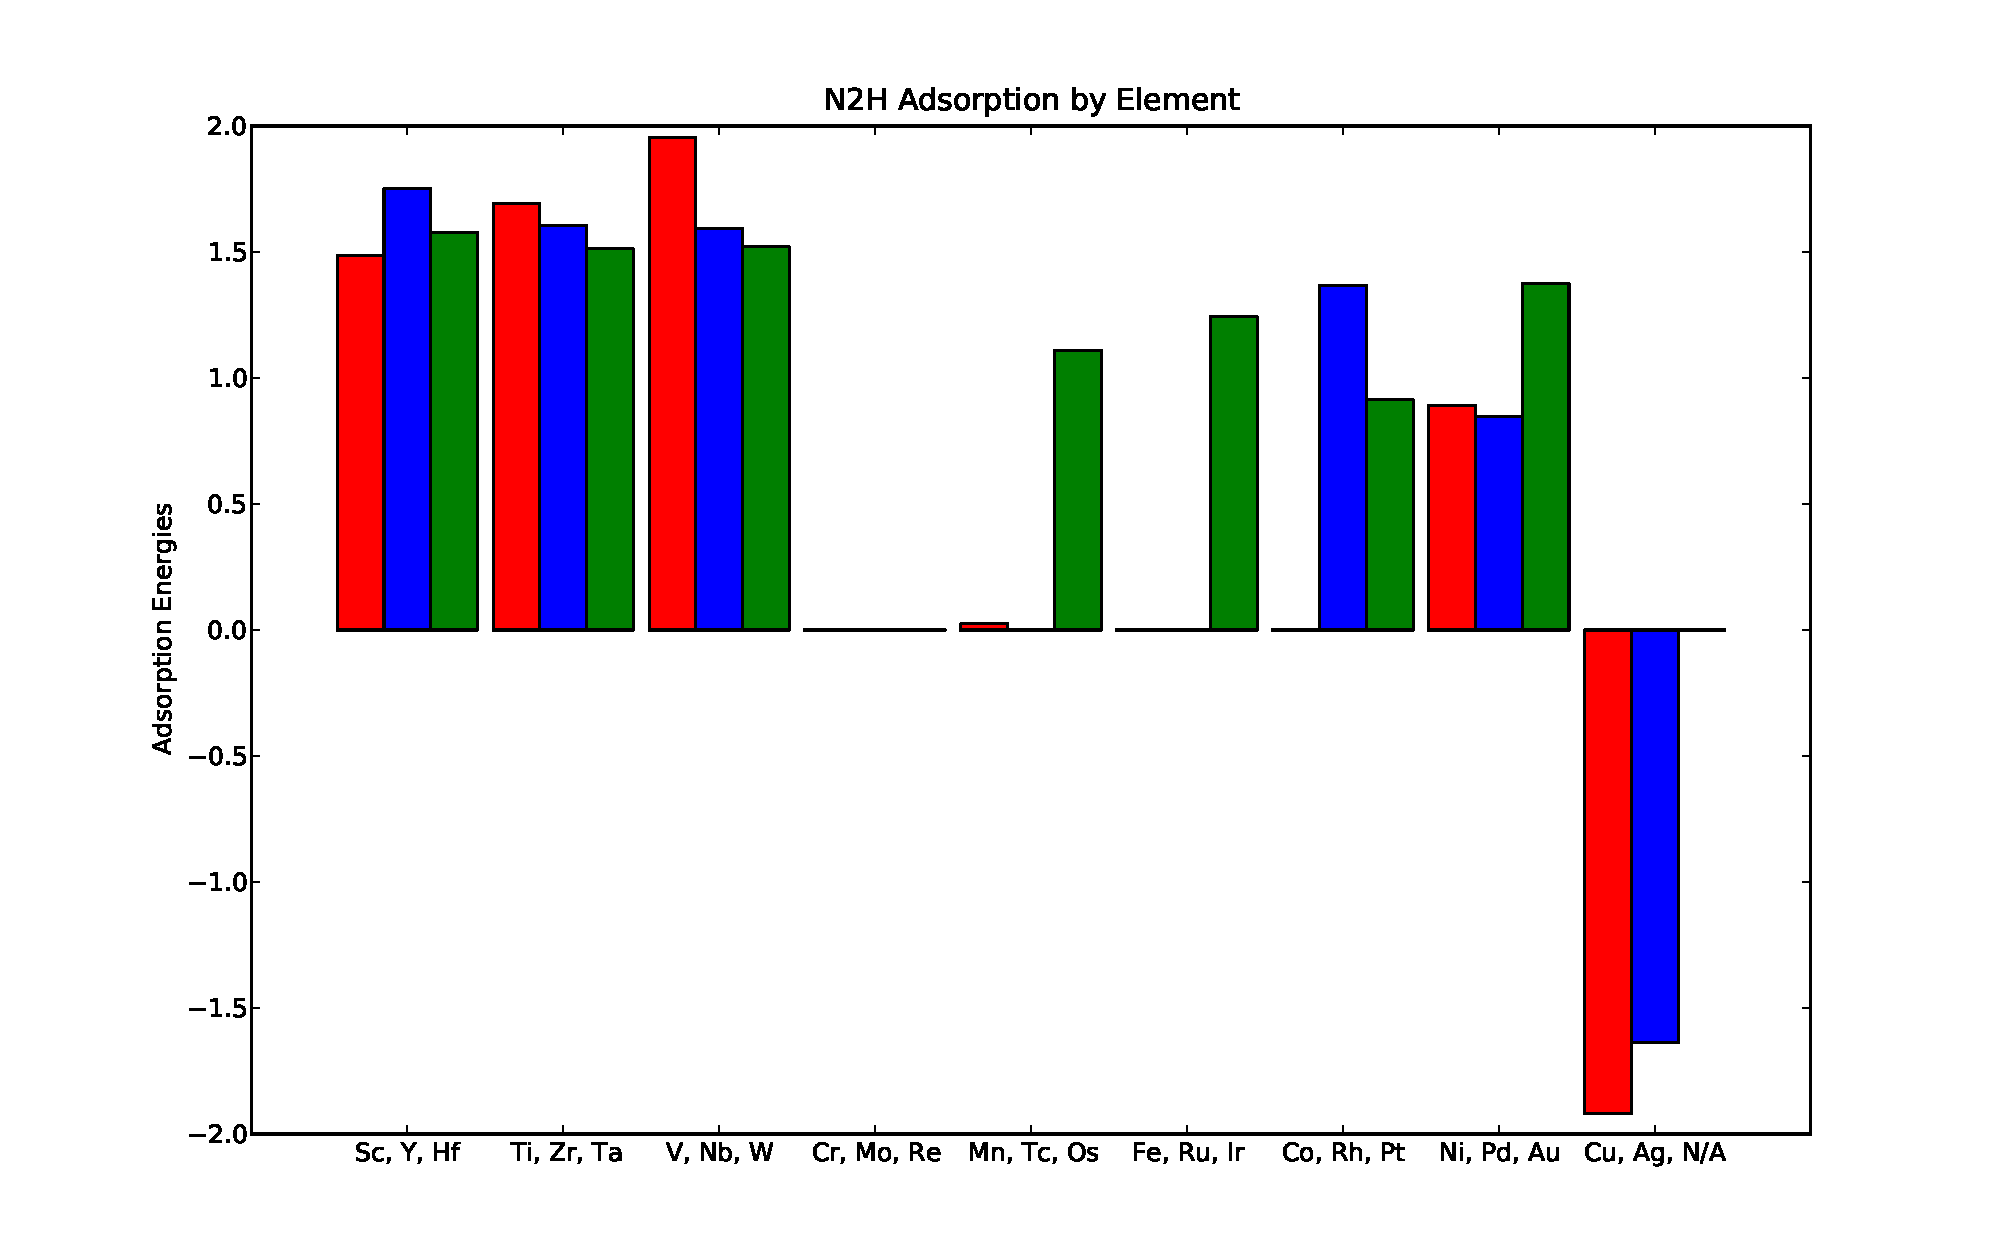
\includegraphics[width=0.8\linewidth]{Images/4+N2H_by_element.pdf}
%    \caption{4+ N2H Adsorption Energy versus Element}
%    \label{fig:4+_N2H_period}
%\end{figure}
%\begin{figure}
%    \centering
%    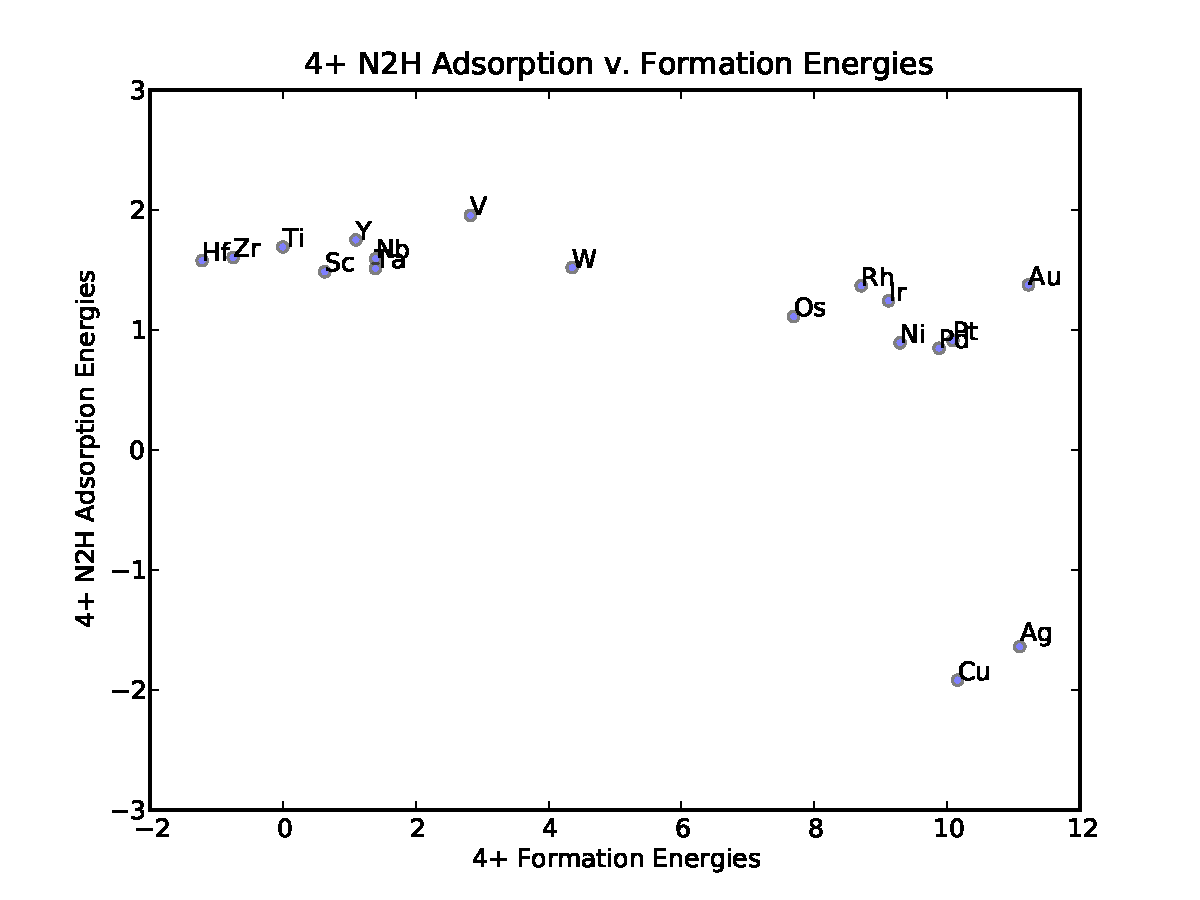
\includegraphics[width=0.8\linewidth]{Images/4+N2H_Formation.pdf}
%    \caption{4+ Formation Energy versus N2H Adsorption Energy}
%    \label{fig:2+_N2H_react_stab}
%\end{figure}

%There is an inherent uncertainty in predicting energies of reactions using DFT. Literature suggests an additional error buffer of around 0.2 eV (CITATIONS). This does not greatly change the interpretation of our results, as the margin of favorability or disfavorability for the calculated reactions is typically larger than 0.2 eV. The change in the likelihood of a reaction occurring with the energetic favorability becomes smaller with increasing magnitude of energies, due to the exponential distribution of temperature.

\subsection{Reactivity Toward Nitrogen Fixation}

The binding energy of N$_2$H has been previously identified to be the primary descriptor for a surface's ability to perform the nitrogen reduction reaction \cite{Hoskuldsson_2017, Montoya_2015}. Thus, to screen surfaces based on their to perform the N$_2$ reduction reaction the N$_2$H binding energies were calculated. From this analysis it was determined that no calculated 4+ sites had N$_2$H states that would allow the nitrogen fixation reaction under ambient conditions, all having N$_2$H binding energies in excess of 1.5eV (see table SXX). However, some 2+ sites has reasonable N$_2$H binding energies thus further thermodynamic pathway analysis was performed for 2+ sites.

The full thermodynamics of the N$_2$ reduction reaction pathways on the 2+ sites were calculated, allowing free energy diagrams to be generated for all possible reaction pathways. All free energy diagrams may be seen in the supplementary information, and the thermodynamic data used to generate these plots may be seen in Table SXX. To assess the nitrogen reduction reaction rates of these sites, two cases were considered: electrochemistry and photochemistry. To simulate electrochemistry, the computational hydrogen electrode model (CHE) was employed. Thus, the effects of applied potential were taken into account with a factor of -eU, where e is the fundamental charge and U is the potential relative to CHE. To simulate the effect of excited electrons, the computational hydrogen electrode was used and the potential was set to that of the band edge of rutile TiO$_2$. %We therefore neglect the effects these metals could have on the photo-physical properties of the material. The free energy diagrams for each pathway considered are available in the supplementary information.

The limiting potential was calculated for all surfaces to asses their ability to reduce N$_2$. The results of this analysis are plotted against the NH$_2$ binding energy in Figure \ref{fig:NH2_limiting_pot}. This plot reveals a volcano type relationship between the NH$_2$ binding energy and the largest barrier of the rate limiting step. Unlike Hoskuldsson et. al.\cite{Hoskuldsson_2017} and Montoya et. al. \cite{Montoya_2015} we find that the NH$_2$ binding energy to be the most powerful descriptor rather than N$_2$H binding, however these quantities are fundamentally linked by scaling relations. We also observe that the limiting step shifts from NH$_2$ desorption on the left to N$_2$ hydrogenation on the right. The only element not following this trend is Ti, whose limiting step is also N$_2$ hydrogenation. This may not be surprising, as electronic interactions between the doping metal and the host metal atoms are known to have an impact on the chemistry of dopant sites, and this particular interaction is absent in the case of Ti \cite{Xu_2015}.\todo{does that make any sense?}. Additionally, Ru and Sc appear to be abnormally unreactive with respect to the trend in the volcano plot.

The two elements lying nearest the top of the volcano are Tc and Co. The former presents a problem for experimental testing, as Tc is a scarce, synthetically produced, radioactive element. In addition, the active sites may be challenging to synthesize due to their relatively high formation energy (see Figure \ref{fig:d_band}). Discouragingly, one of the species also near the top of the volcano is the host metal of the oxide material, Ti. This means that substituting other metals will only yield moderate improvements on rates of reaction for electrocatalysis. However, Co lowers limiting potential by 0.2V and is inexpensive and abundant making it a good candidate for experimental investigation.


To examine the ability of dopant metals to improve photocatalytic nitrogen reduction, a potential was applied equivalent to the potential of excited electrons at the band edge (approximately -0.15V). The highest thermodynamic barrier for the best reaction pathway plotted vs the NH$_2$* binding energy may be seen in Figure \ref{fig:NH2_limiting_bar}. It should be noted that this quantity is different than the limiting potential, as it includes non-electrochemical steps in addition to electrochemical steps. A potential equal to the band edge is also applied (-0.15V for rutile) to simulate the effect of excited electrons. This improves the thermodynamics of the electrochemical steps, while leaving the surface steps unchanged. Because the energy of the NH$_3$* state is roughly equal to that of the NH$_2$* for most studied metals modifying the potential has a limited effect on metals on the left side of the plot. This is because the desorption of NH$_2$ (a non-electrochemical step) rapidly becomes rate limiting. The primary effect this has is to shift surfaces with in which the limiting step is N$_2$ hydrogenation to be more favorable, effectively shifting the entire right side of the volcano downward. This moves Co to have a maximum thermodynamic barrier of ~0.85eV, making photocatalysis at room temperature feasible.

The lack of improvement in the rate of reaction with the addition of Ru, Pt, and Pd in the case of photocatalysis also agrees with the previous experimental findings by Hirakawa et. al.\cite{Hirakawa_2017}. They report no improvements in reaction rates when metals are bound to the TiO$_2$ surface.


\begin{figure}
    \centering
    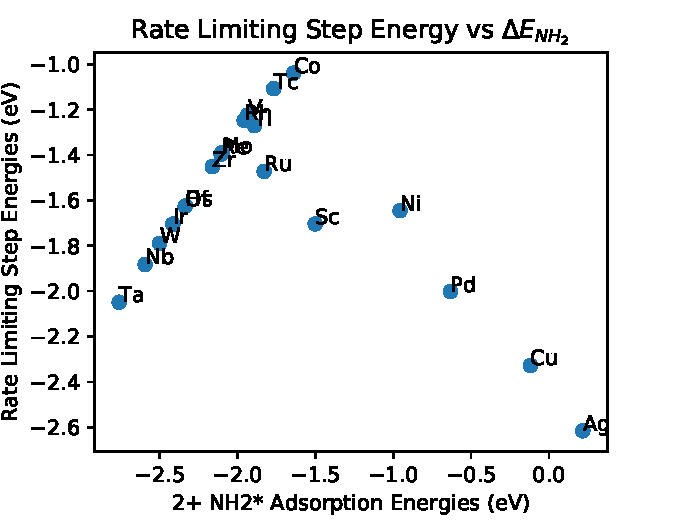
\includegraphics[width=0.4\textwidth]{Images/NH2_v_limiting_pot.pdf}
    
    \caption{The limiting potential vs the NH$_2$ Binding Energy}
    \label{fig:NH2_limiting_pot}
\end{figure}

These results highlight the challenge of improving reaction rates for nitrogen fixation, indicating that more creative strategies must be employed. While have not considered the possible effects of metals on TiO$_2$'s bulk photochemical properties such as charge separation and carrier lifetime we believe this provides a starting point for engineering surface segregated metal dopants. In future, we could imagine engineering oxide structures with metal dopants in the bulk structure that improve photochemical properties and surface segregated metal dopants that improve reaction kinetics.

\begin{figure}
    \centering
    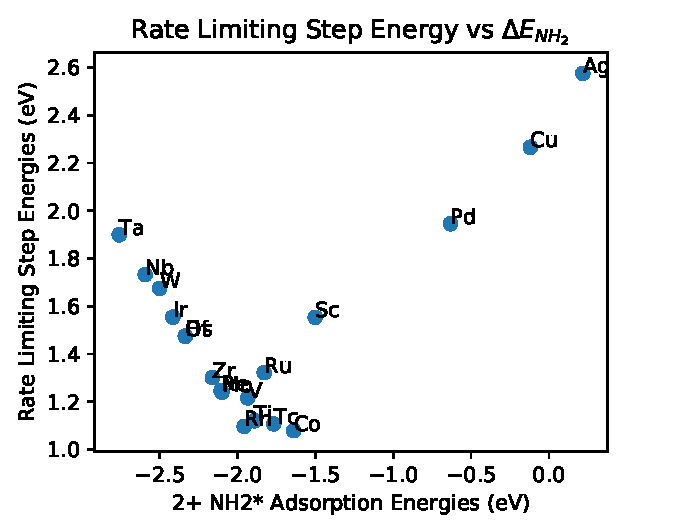
\includegraphics[width=0.4\textwidth]{Images/NH2_v_rate_limiting.pdf}
    
    \caption{The highest barrier observed vs the NH$_2$ Binding Energy}
    \label{fig:NH2_limiting_bar}
\end{figure}

\section{Conclusions}
This work has investigated stability of metal dopant surface sites and their effects on the reaction thermodynamics of N$_2$ reduction on rutile (110). We find that the formation energy of these doped surface states is strongly related to the location of the \textit{d}-band center of the subsituted metal, with the trend matching the \textit{d}-band model. We also find correlation between the cohesive energy of metals and their N$_2$H and NH$_2$ binding energy on the surface, suggesting that the bonding and anti-bonding regions of \textit{d}-band lies close to the fermi level. Finally, we investigate the effects of dopant sites on the full reaction pathways for 2+ sites on all studied metals. We find a volcano type relationship between NH$_2$ binding and the highest reaction barrier in the pathway for photocatalytic rations. We find that the formation of Co 2+ sites would yield an improvement of reaction rates in electrocatalysis and photocatalysis. We also show that metal dopant sites possess a substantial ability to modify reaction thermodynamics on the surface. For this reason, generating metal dopant sites on the surface is a potential path forward for improving reaction rates on metal oxide surfaces.


\section{Methods}
\label{sec:methods}

\subsection{Density Functional Theory Calculations}
All first principles calculations were performed in the Quantum Espresso software package \cite{QE-2009}.
The TiO$_2$ slabs and atomistic images were created using the Atomic Simulation Environment (ASE) package\cite{Hjorth_Larsen_2017}. The surfaces were constructed with 4 TiO$_2$ tri-layers, with a 1x2 supercell repeat. The pristine slab totals 48 atoms, with 4 Ti and 8 O per tir-layer. To generate the 2+ doped TiO$_2$ slabs, a 6-fold Ti atom was replaced with a subsitutent metal and one bridging O was removed to create a vacancy. 6 Angstroms of vacuum were added on both top and bottom of the slab and dipole corrections were applied, to avoid adverse effects of periodicity in the z direction. The lattice parameters of the unit cells were fixed at the calculated value for pure rutile TiO$_2$. Spin polarization was implemented in all simulations to ensure the lowest energy spin state was obtained for each site.

For the DFT calculations, the bottom 4 Ti and 14 O atoms were fixed in bulk positions. A plane wave cutoff of 400 eV and a Monkhorst-Pack k-point grid with a spacing of 4x4x1 was used \cite{Monkhorst_1976}. Dipole corrections and spin polarization were included, and the magnetic moments were perturbed for each calculation. The convergence threshold was selected as $10^{-6}$ eV, and BEEF-vdW functionals \cite{Wellendorff_2012} with Fermi-Dirac smearing were used.

The adsorption energies were obtained from the DFT calculations by subtracting the energy of a clean slab and the energy of the free gas molecule from the energy of the gas adsorbed to the slab. 
\begin{equation}
E_{adsorption} = E_{slab+adsorbate} - E_{slab} - E_{adsorbate}
\end{equation}
%The error of DFT calculations tends to be in the order of magnitude of 0.5 eV \cite{Gautier_2015}. 

\subsection{Thermochemistry}
\cite{ase-paper,Reuter_2005}

To calculate the adsorption energy at standard temperature and pressure, the Thermochemistry package from ASE was used \cite{ase-paper}. Free gasses were approximated in the ideal gas limit, and adsorbed gasses in the harmonic limit. The ideal gas limit thermochemistry allows translation and rotation in all directions, and assumes these modes are independent. The harmonic limit thermochemistry module approximates vibrations in all directions as harmonic oscillators. From these results, the free energies were calculated using Equation \ref{eq:gibbs} The vibrational mode for all metals were assumed to be approximately the same as those of the repective species adsorbed to the oxygen vacant TiO$_2$ (110) surface, thus the same thermodynamic correction values were applied to all species of the same type.
\begin{equation}
    G=H-TS
    \label{eq:gibbs}
\end{equation}. 

\subsection{Photochemistry}
The photochemistry has been treated using the methods outlined by Hellman et. al. \cite{Hellman2017}. Within this framework, the effects of excited states are neglected allowing the treatment of excited electrons and holes using the computational hydrogen electrode model (CHE). The potentials of electrons and holes are set at the value of the band edges of the semiconductor.

\section{Acknowledgements}
We would like to thank Fuhzu Liu and Gabriel Gusm\~ao for their comments and suggestions for improving this manuscript.

\bibliographystyle{abbrv}
\bibliography{main}
Supplementary Information
\onecolumn
\begin{table}
\begin{center}
\begin{tabular}{| c | c | c | c | c | c | c | c | c | c | c | c | c | c |}
\hline
Element & H$_2$NNH$_2$ & HNNH & N & N$_2$ & N$_2$H & N$_2$H$_2$ & N$_2$H$_3$ & NH & NH$_2$ & NH$_3$ & Formation Energy\\
\hline

Rh & 1.16 & 1.3 & 1.86 & -0.16 & 0.71 & 0.85 & 0.44 & 1.34 & -0.88 & -0.87 & 6.01 \\
Ir & 0.82 & 0.74 & 1.03 & -0.7 & 0.26 & 0.19 & -0.01 & 0.54 & -1.34 & -1.2 & 7.07 \\
Ru & 0.82 & 0.76 & 0.48 & -0.83 & 0.64 & 0.17 & 0.57 & 0.86 & -0.76 & -1.13 & 5.45 \\
W & 1.25 & 0.84 & -1.8 & -0.37 & -0.24 & -0.73 & 0.01 & -1.06 & -1.43 & -0.8 & 3.99 \\
Tc & 1.03 & 0.95 & -0.87 & -0.65 & 0.06 & 0.27 & 0.65 & 0.52 & -0.69 & -0.92 & 4.58 \\
Zr & 1.23 & 1.39 & 1.71 & -0.01 & 1.07 & 0.74 & 0.35 & 0.16 & -1.09 & -0.88 & -0.51 \\
Re & 0.95 & 0.67 & -1.5 & -0.83 & -0.42 & -0.15 & 0.32 & -0.18 & -1.03 & -0.96 & 5.06 \\
Pd & 1.53 & 2.12 & 3.55 & 0.23 & 2.0 & 2.25 & 1.67 & 2.5 & 0.44 & -0.22 & 6.08 \\
Ti & 1.42 & 1.64 & 1.73 & 0.11 & 1.27 & 0.85 & 0.61 & 0.37 & -0.82 & -0.6 & 0.0 \\
Cu & 1.33 & 2.07 & 4.51 & 0.18 & 2.33 & 2.4 & 1.65 & 3.41 & 0.95 & -0.45 & 6.55 \\
Ni & 1.75 & 1.94 & 3.35 & 0.17 & 1.64 & 1.9 & 1.09 &  & 0.12 & -0.43 & 5.58 \\
Os & 0.61 & 0.39 & -0.7 & -1.17 & -0.15 & -0.36 & 0.06 & 0.06 & -1.26 & -1.29 & 6.31 \\
Ta & 1.1 & 0.31 & -0.99 & -0.13 & 0.42 & -0.32 & -0.22 & -0.95 & -1.69 & -0.85 & 1.69 \\
Hf & 1.21 & 1.32 & 1.59 & -0.02 & 0.97 & 0.6 & 0.2 & 0.02 & -1.26 & -0.95 & -0.92 \\
Sc & 1.06 & 1.76 & 3.51 & 0.03 & 1.7 & 1.59 & 1.0 & 2.18 & -0.43 & -0.76 & -1.71 \\
Co & 1.14 & 1.53 & 2.34 & 0.12 & 1.04 & 1.05 & 0.78 & 1.82 & -0.57 & -0.72 & 4.49 \\
V & 1.43 & 1.5 & -0.33 & 0.04 & 0.82 & 0.38 & 0.55 & 0.17 & -0.86 & -1.03 & 2.48 \\
Y & 1.01 & 1.69 & 2.72 & 0.02 &  & 2.0 & 1.34 & 2.58 & 0.02 & -0.77 & -1.38 \\
Au & 1.68 & 2.36 & 4.05 & 0.25 & 2.54 & 2.82 & 2.15 & 2.95 & 0.92 & -0.08 & 8.18 \\
Mo & 1.27 & 1.11 & -1.2 & -0.33 & 0.01 & -0.08 & 0.39 & -0.24 & -1.03 & -0.75 & 3.26 \\
Ag & 1.44 & 2.33 & 5.3 & 0.24 & 2.62 & 2.65 & 2.04 & 3.83 & 1.29 & -0.18 & 7.28 \\
Pt &  & 2.16 & 2.77 & 0.26 & 1.78 & 2.06 & 1.44 & 1.69 & 0.08 & -0.09 & 6.86 \\
Nb & 1.23 & 0.43 & -1.04 & -0.23 & 0.35 & -0.36 & -0.04 & -0.84 & -1.52 & -0.86 & 1.5 \\
\hline
\end{tabular}
\end{center}
\caption{The calculated relative energies of all 2+ surface species on all metal substituents at standard state. All energies are referenced with respect to N$_2$ gas and H$_2$ gas at 300K and 1 bar of pressure. Blank spaces represent calculations that could not be converged}
\label{table:energies}
\end{table}

\begin{table}
\begin{center}
\begin{tabular}{| c | c | c | c |}
\hline
Element & N$_2$ & N$_2$H & Formation Energy \\
\hline
Rh & -0.14 & 2.22 & 8.71 \\
Ir & -0.39 & 2.1 & 9.12 \\
Ru & -0.0 &  & 7.5 \\
W & 0.13 & 2.37 & 4.36 \\
Tc & 0.12 &  & 5.88 \\
Zr & 0.07 & 2.46 & -0.75 \\
Re & 0.12 &  & 5.9 \\
Pd & -0.01 & 1.7 & 9.88 \\
Fe & -0.12 &  & 8.4 \\
Ti & 0.16 & 2.54 & -0.0 \\
Cu & 0.22 &  & 10.16 \\
Ni & 0.2 & 1.75 & 9.29 \\
Os & -0.22 & 1.96 & 7.69 \\
Ta & 0.1 & 2.37 & 1.39 \\
Hf & 0.06 & 2.43 & -1.22 \\
Sc & 0.08 & 2.34 & 0.63 \\
Co & 0.2 &  & 7.42 \\
V & 0.19 & 2.81 & 2.82 \\
Y & 0.04 & 2.6 & 1.1 \\
Au & 0.27 & 2.23 & 11.22 \\
Mo & 0.14 &  & 3.95 \\
Ag & 0.24 &  & 11.09 \\
Pt & -0.34 & 1.77 & 10.08 \\
Nb & 0.11 & 2.45 & 1.4 \\
\hline
\end{tabular}
\end{center}
\caption{The calculated relative energies of all 4+ surface species on all metal substituents at standard state. All energies are referenced with respect to N$_2$ gas and H$_2$ gas at 300K and 1 bar of pressure. Blank spaces represent calculations that could not be converged}
\hline
\end{table}

\begin{table}
\begin{center}
\begin{tabular}{| c | c |c |}
\hline
Element & Limiting Potential & Limiting Step \\
\hline
Sc & -1.7 & N$_2$ $\rightarrow$ N$_2$H*\\
Ti & -1.27 & N$_2$ $\rightarrow$ N$_2$H*\\
V & -0.82 & N$_2$ $\rightarrow$ N$_2$H*\\
Co & -1.04 & N$_2$ $\rightarrow$ N$_2$H*\\
Ni & -1.64 & N$_2$ $\rightarrow$ N$_2$H*\\
Cu & -2.33 & N$_2$ $\rightarrow$ N$_2$H*\\
Zr & -1.08 & N$_2$* $\rightarrow$ N$_2$H*\\
Nb & -1.38 & NH$_2$*+NH$_3$ $\rightarrow$ 2NH$_3$\\
Mo & -0.89 & NH$_2$*+NH$_3$ $\rightarrow$ 2NH$_3$\\
Tc & -0.71 & N$_2$* $\rightarrow$ N$_2$H*\\
Ru & -1.47 & N$_2$* $\rightarrow$ N$_2$H*\\
Rh & -0.88 & N$_2$* $\rightarrow$ N$_2$H*\\
Pd & -2.0 & N$_2$ $\rightarrow$ N$_2$H*\\
Ag & -2.62 & N$_2$ $\rightarrow$ N$_2$H*\\
Hf & -1.12 & NH$_2$*+NH$_3$ $\rightarrow$ 2NH$_3$\\
Ta & -1.55 & NH$_2$*+NH$_3$ $\rightarrow$ 2NH$_3$\\
W & -1.29 & NH$_2$*+NH$_3$ $\rightarrow$ 2NH$_3$\\
Re & -0.9 & NH$_2$*+NH$_3$ $\rightarrow$ 2NH$_3$\\
Os & -1.12 & NH$_2$*+NH$_3$ $\rightarrow$ 2NH$_3$\\
Ir & -1.2 & NH$_2$*+NH$_3$ $\rightarrow$ 2NH$_3$\\
Au & -2.48 & N$_2$ $\rightarrow$ N$_2$H*\\
\hline
\end{tabular}
\end{center}
\caption{The limiting potentials and limiting steps for each dopant metal on 2+ surfaces}\label{table:limiting_steps}\end{table}\hline
\end{table}

\begin{table}
\begin{center}
\begin{tabular}{| c | c |c |}
\hline
Element & Limiting Potential & Limiting Step \\
\hline
Sc & 0.44 & NH$_3$*+NH$_3$ $\rightarrow$ 2NH$_3$\\
Ti & 0.68 & NH$_3$*+NH$_3$ $\rightarrow$ 2NH$_3$\\
V & 0.72 & NH$_3$*+NH$_3$ $\rightarrow$ 2NH$_3$\\
Co & 0.43 & NH$_3$*+NH$_3$ $\rightarrow$ 2NH$_3$\\
Ni & 0.17 & N$_2$ $\rightarrow$ N$_2$*\\
Cu & 1.25 & H$_2$NNH$_2$* $\rightarrow$ 2NH$_2$*\\
Zr & 0.95 & NH$_3$*+NH$_3$ $\rightarrow$ 2NH$_3$\\
Nb & 1.38 & NH$_3$*+NH$_3$ $\rightarrow$ 2NH$_3$\\
Mo & 0.89 & NH$_3$*+NH$_3$ $\rightarrow$ 2NH$_3$\\
Tc & 0.61 & NH$_3$*+NH$_3$ $\rightarrow$ 2NH$_3$\\
Ru & 0.82 & NH$_3$*+NH$_3$ $\rightarrow$ 2NH$_3$\\
Rh & 0.75 & NH$_3$*+NH$_3$ $\rightarrow$ 2NH$_3$\\
Pd & 0.54 & H$_2$NNH$_2$* $\rightarrow$ 2NH$_2$*\\
Ag & 1.48 & H$_2$NNH$_2$* $\rightarrow$ 2NH$_2$*\\
Hf & 1.12 & NH$_3$*+NH$_3$ $\rightarrow$ 2NH$_3$\\
Ta & 1.55 & NH$_3$*+NH$_3$ $\rightarrow$ 2NH$_3$\\
W & 1.29 & NH$_3$*+NH$_3$ $\rightarrow$ 2NH$_3$\\
Re & 0.9 & NH$_3$*+NH$_3$ $\rightarrow$ 2NH$_3$\\
Os & 1.12 & NH$_3$*+NH$_3$ $\rightarrow$ 2NH$_3$\\
Ir & 1.2 & NH$_3$*+NH$_3$ $\rightarrow$ 2NH$_3$\\
Au & 0.82 & H$_2$NNH$_2$* $\rightarrow$ 2NH$_2$*\\
\hline
\end{tabular}
\end{center}
\caption{The largest thermodynamic barrier and correspinding steps for each dopant metal on 2+ surfaces}\label{table:limiting_steps}\end{table}\begin{figure}
\centering
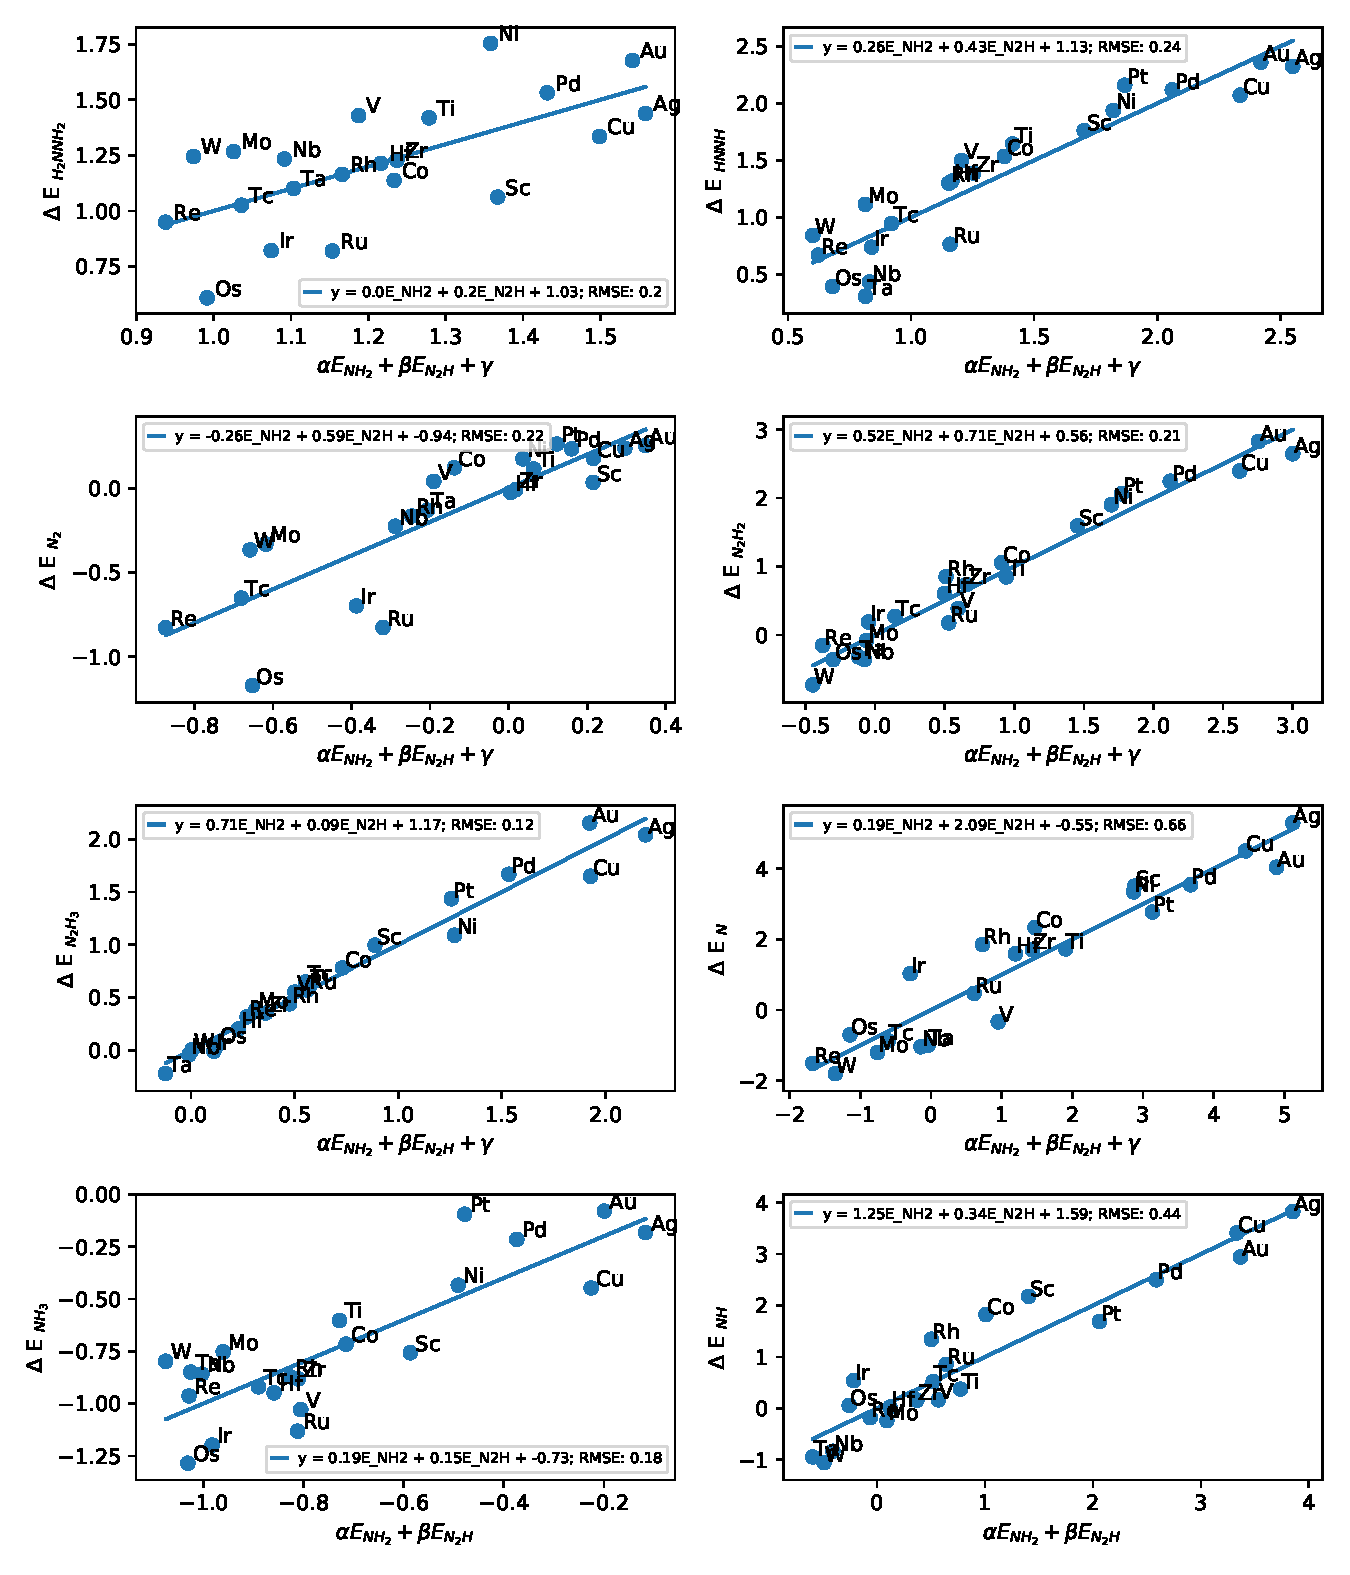
\includegraphics[width=0.8\linewidth]{Images/scaling_species.pdf}
\caption{The calculated scaling relations between the binding energies of various species and the binding energies of N$_2$H and NH$_2$ on 2+ dopant sites}
\end{figure}

\begin{figure}
\centering
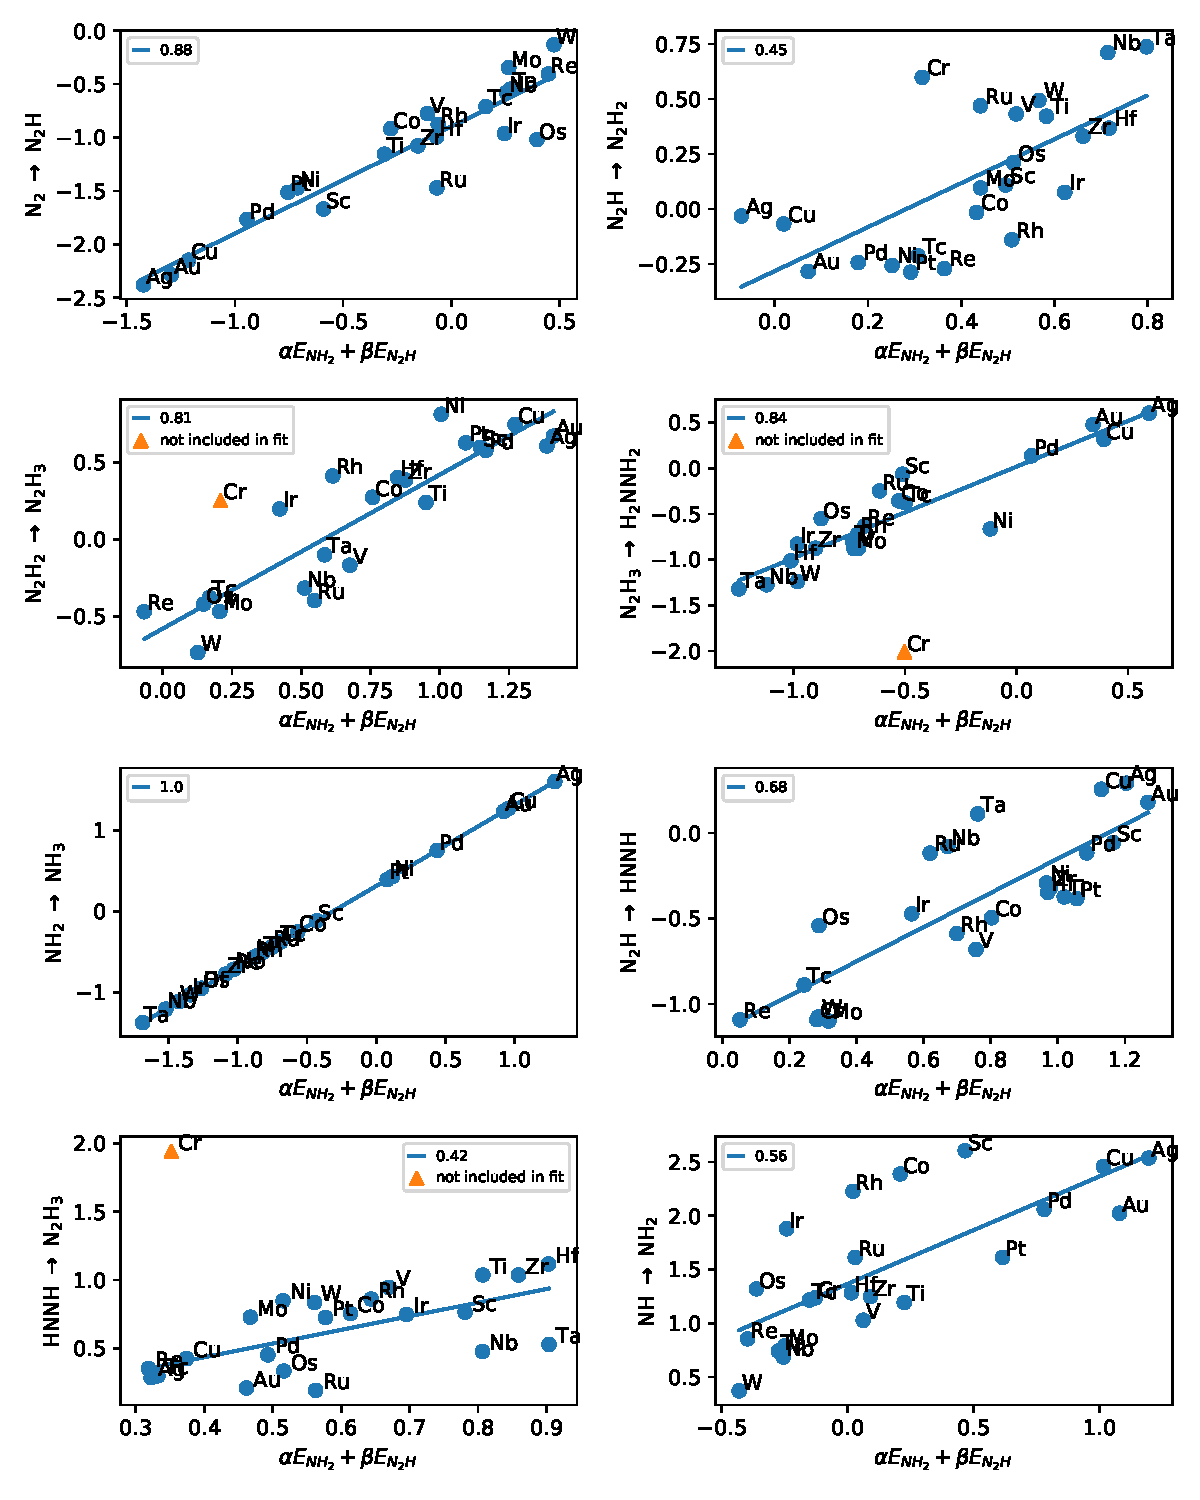
\includegraphics[width=0.8\linewidth]{Images/scaling_reactions.pdf}
\caption{The calculated scaling relations between the binding energies of various species and the binding energies of N$_2$H and NH$_2$ on 2+ dopant sites}
\end{figure}

\begin{figure}
\centering
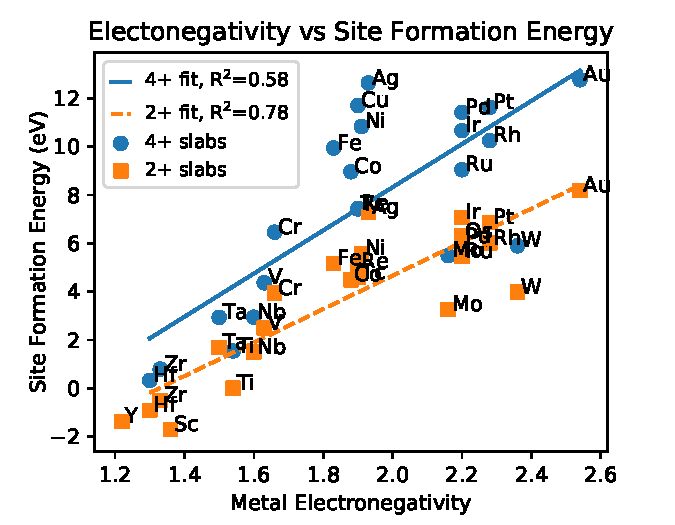
\includegraphics[width=0.8\linewidth]{Images/electronegativity_vs_formation.pdf}
\caption{Electronegativity vs formation energy of 2+ dopant site}
\end{figure}

\begin{figure}
\centering
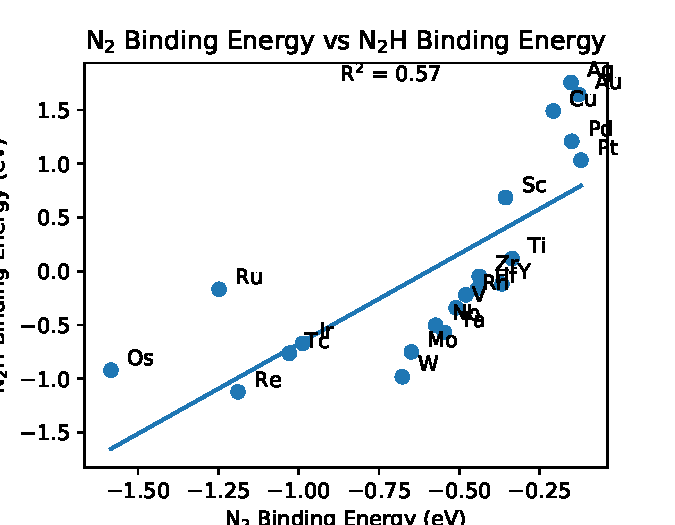
\includegraphics[width=0.8\linewidth]{Images/N2_vs_N2H.pdf}
\caption{The binding energy of N$_2$ vs N$_2$H}
\end{figure}

\begin{figure}
\centering
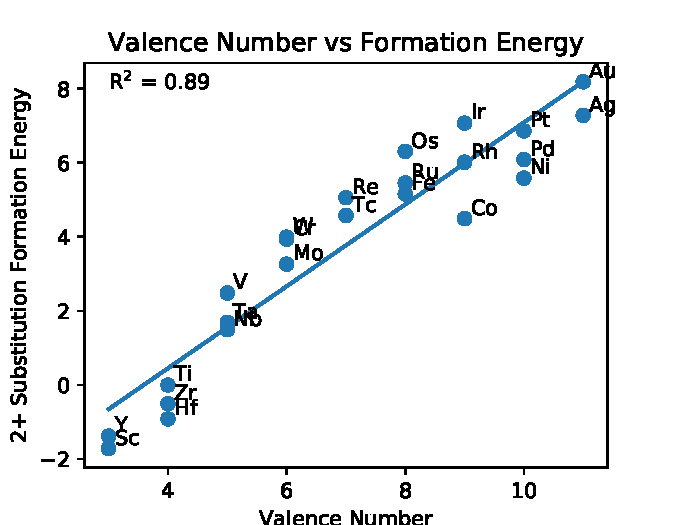
\includegraphics[width=0.8\linewidth]{Images/Valence_vs_formation_energy.pdf}
\caption{Valence number vs formation energy of 2+ dopant site}
\end{figure}

\begin{figure}
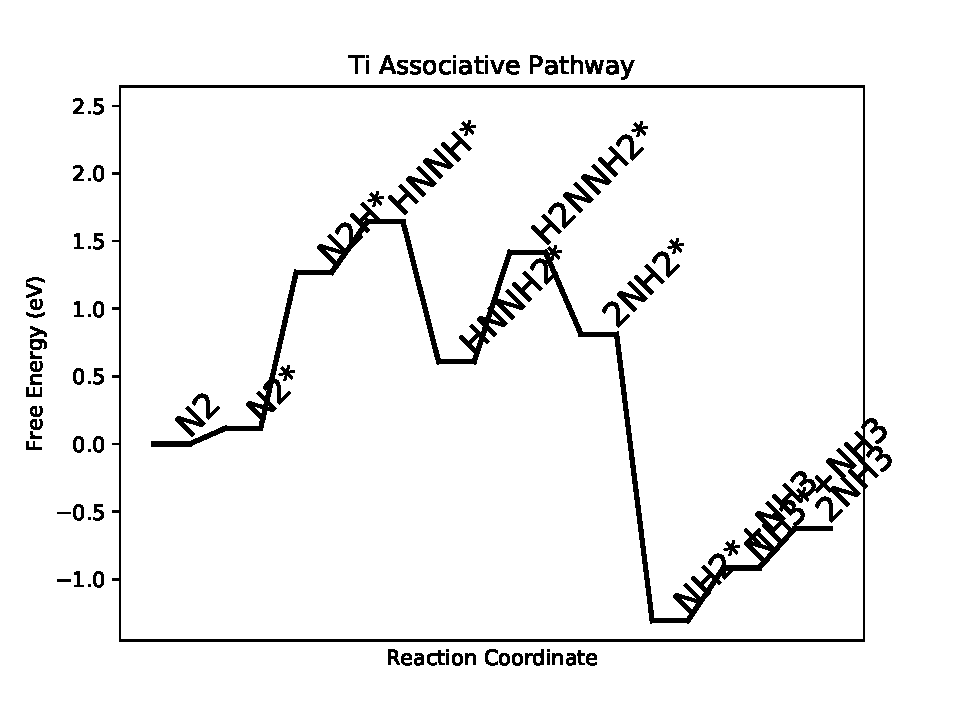
\includegraphics[width=0.8\linewidth]{data/plots/Ti_associative.pdf}
\end{figure}

\begin{figure}
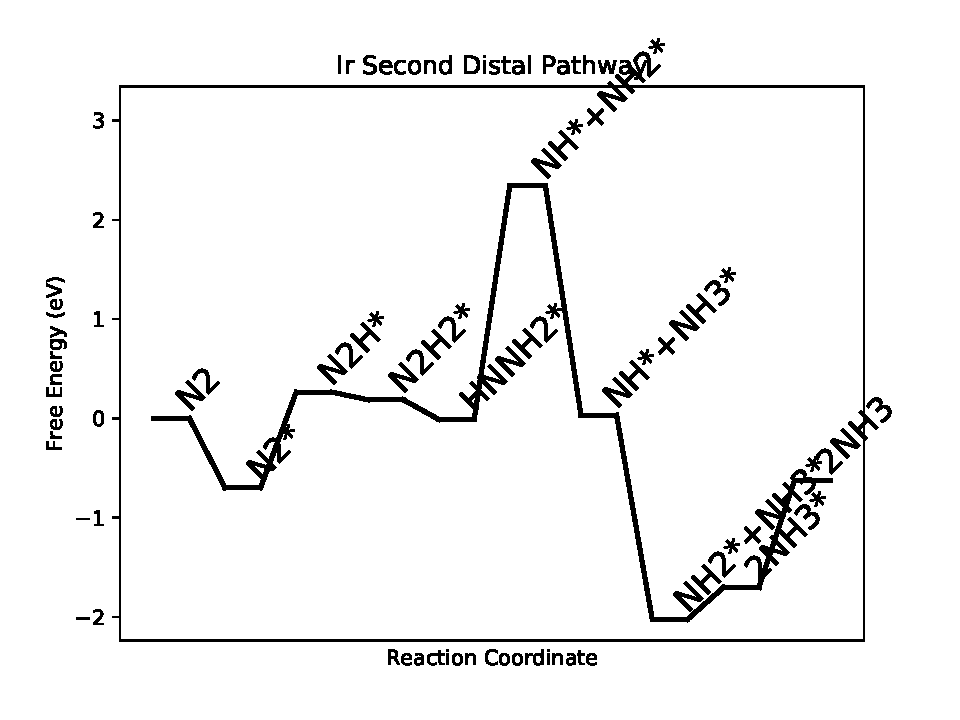
\includegraphics[width=0.8\linewidth]{data/plots/Ir_distal_2.pdf}
\end{figure}

\begin{figure}
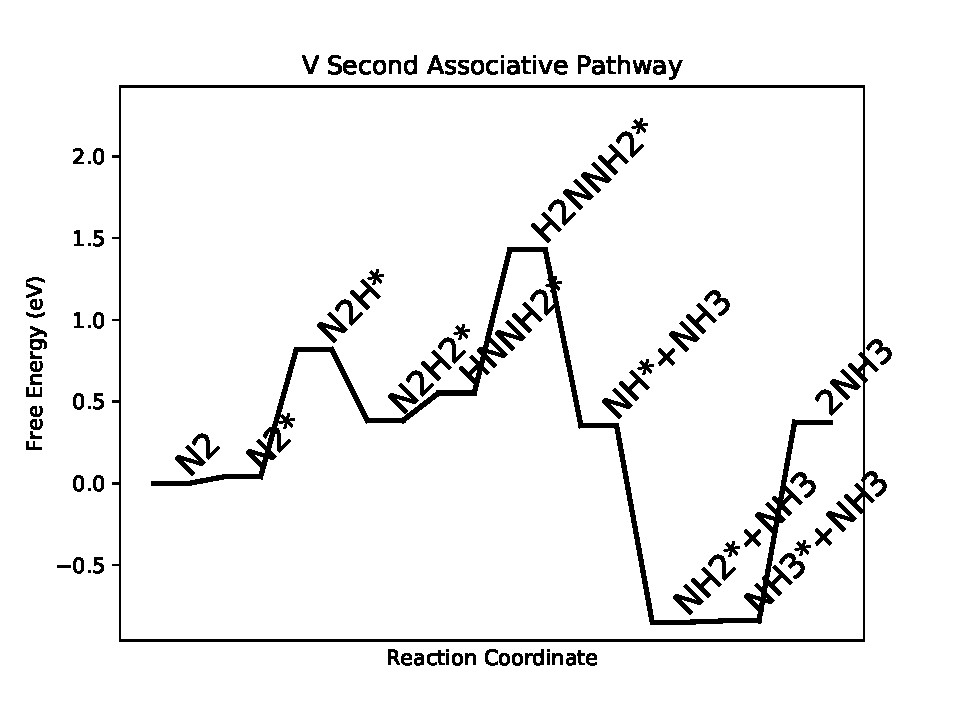
\includegraphics[width=0.8\linewidth]{data/plots/V_associative_2.pdf}
\end{figure}

\begin{figure}
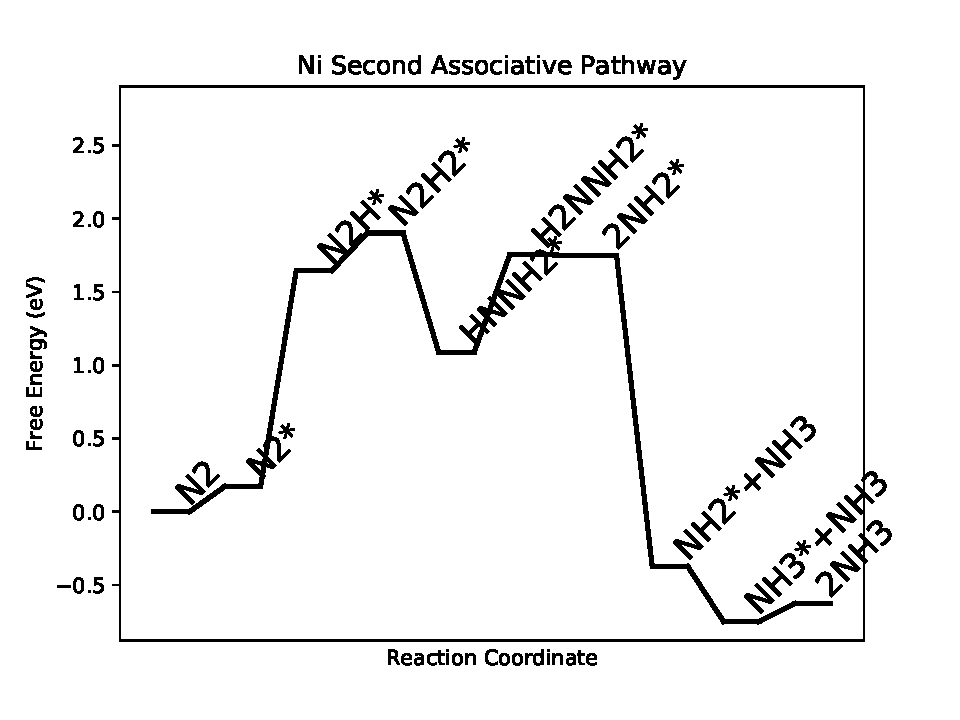
\includegraphics[width=0.8\linewidth]{data/plots/Ni_associative_2.pdf}
\end{figure}

\begin{figure}
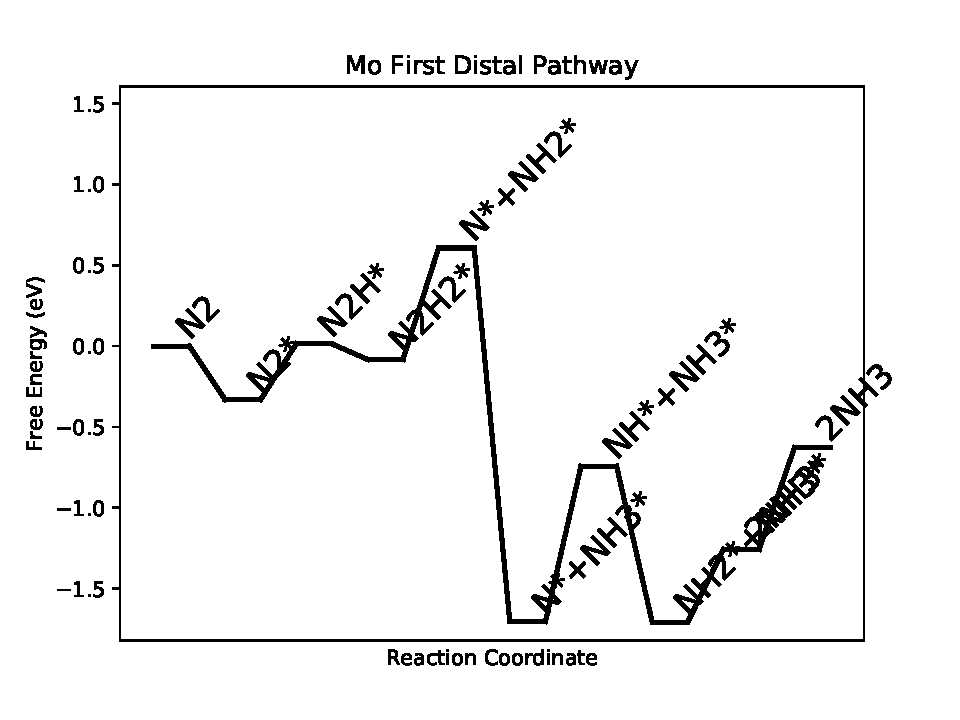
\includegraphics[width=0.8\linewidth]{data/plots/Mo_distal_1.pdf}
\end{figure}

\begin{figure}
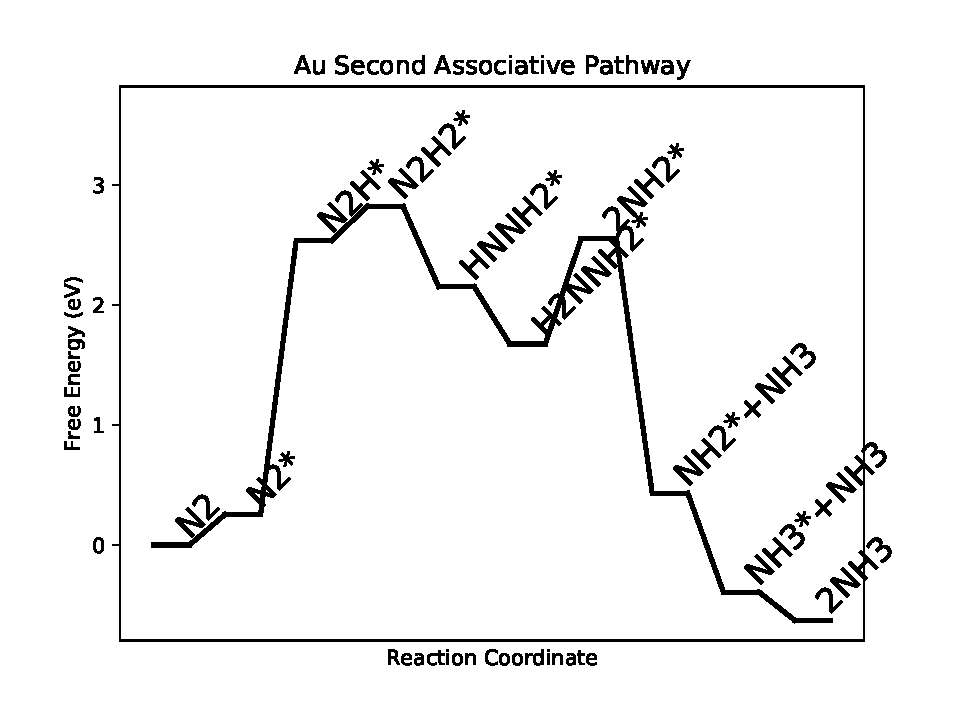
\includegraphics[width=0.8\linewidth]{data/plots/Au_associative_2.pdf}
\end{figure}

\begin{figure}
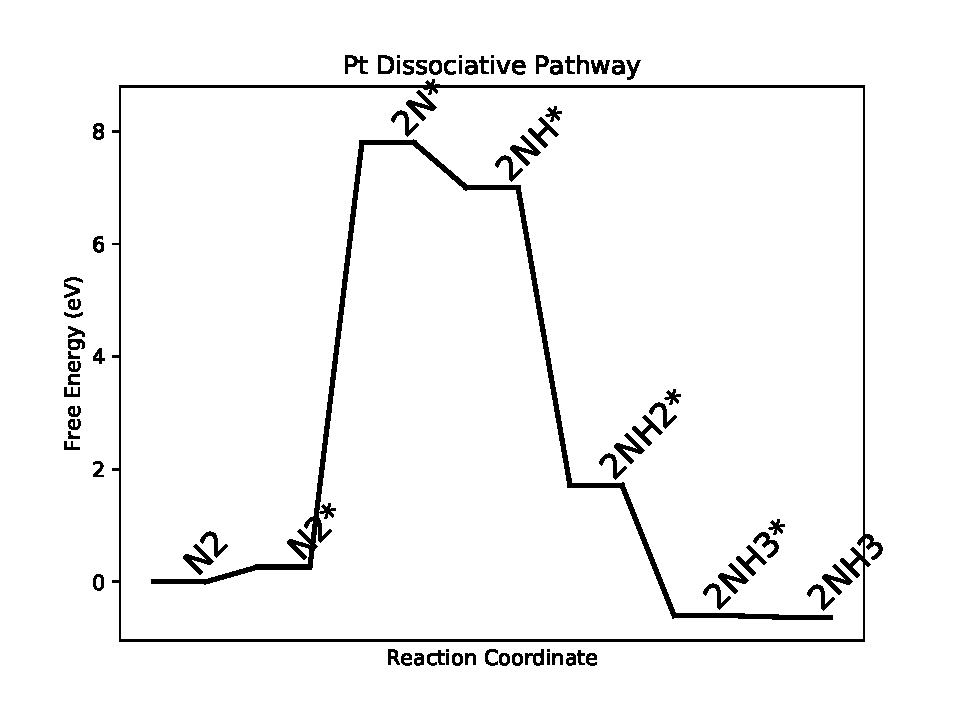
\includegraphics[width=0.8\linewidth]{data/plots/Pt_dissociative.pdf}
\end{figure}

\begin{figure}
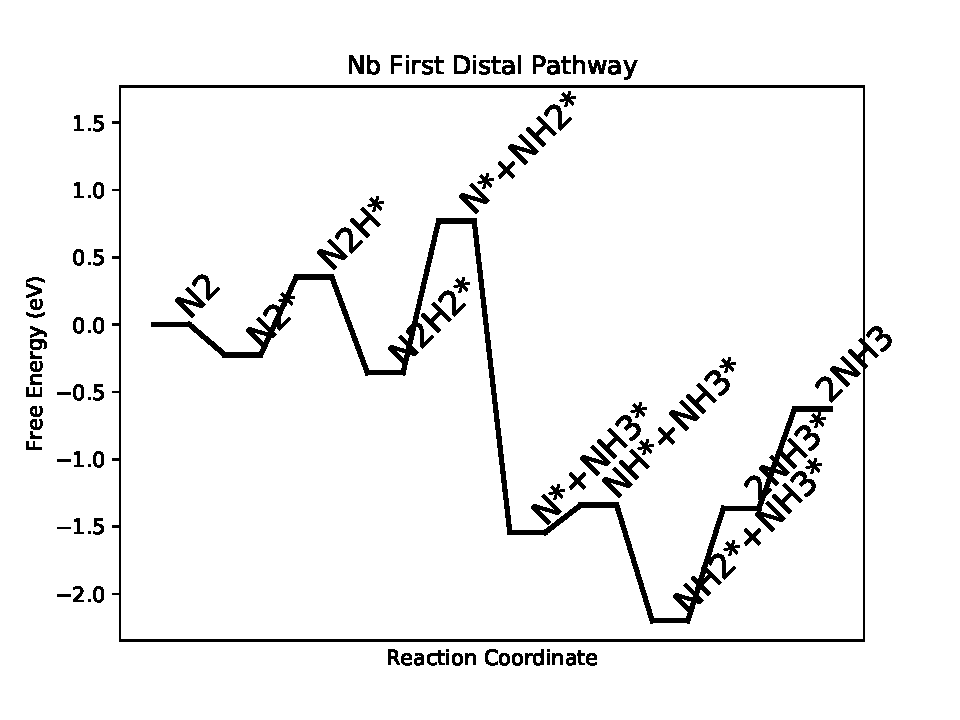
\includegraphics[width=0.8\linewidth]{data/plots/Nb_distal_1.pdf}
\end{figure}

\begin{figure}
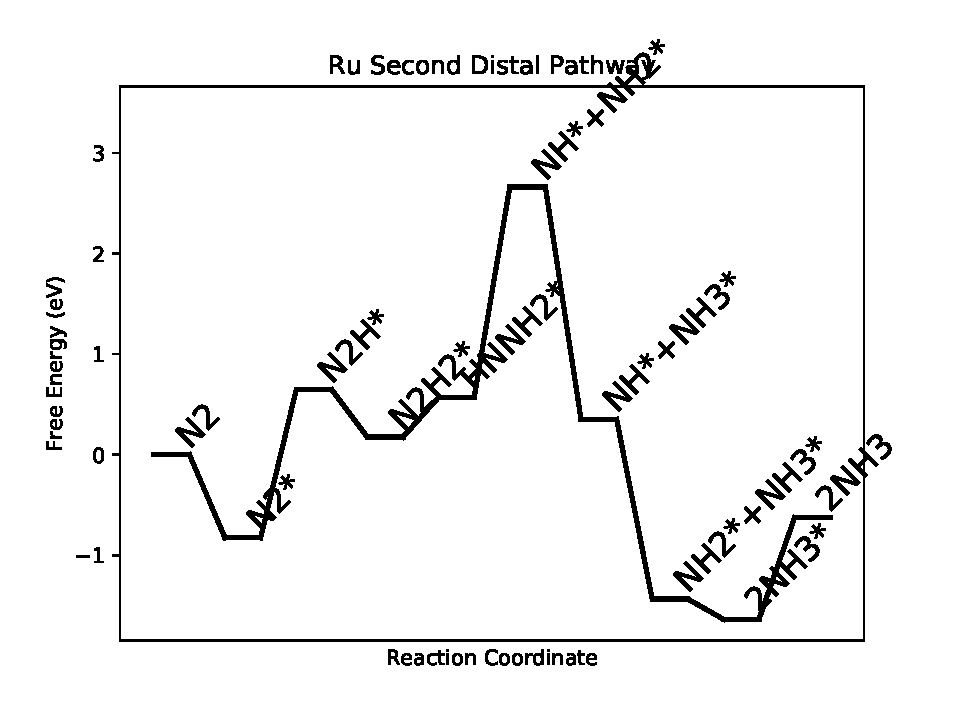
\includegraphics[width=0.8\linewidth]{data/plots/Ru_distal_2.pdf}
\end{figure}

\begin{figure}
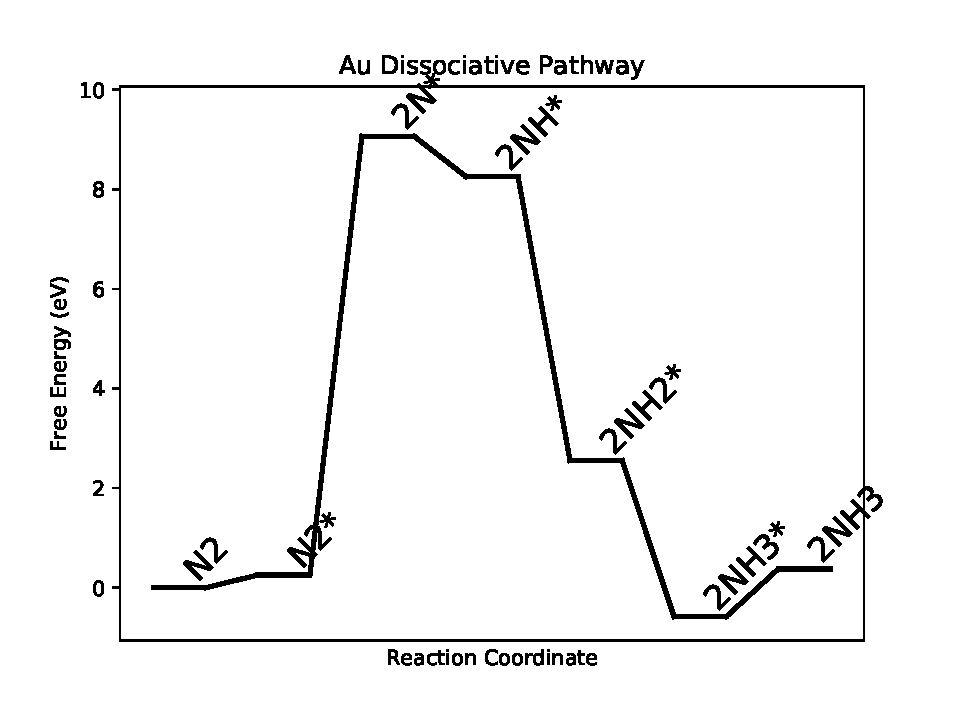
\includegraphics[width=0.8\linewidth]{data/plots/Au_dissociative.pdf}
\end{figure}

\begin{figure}
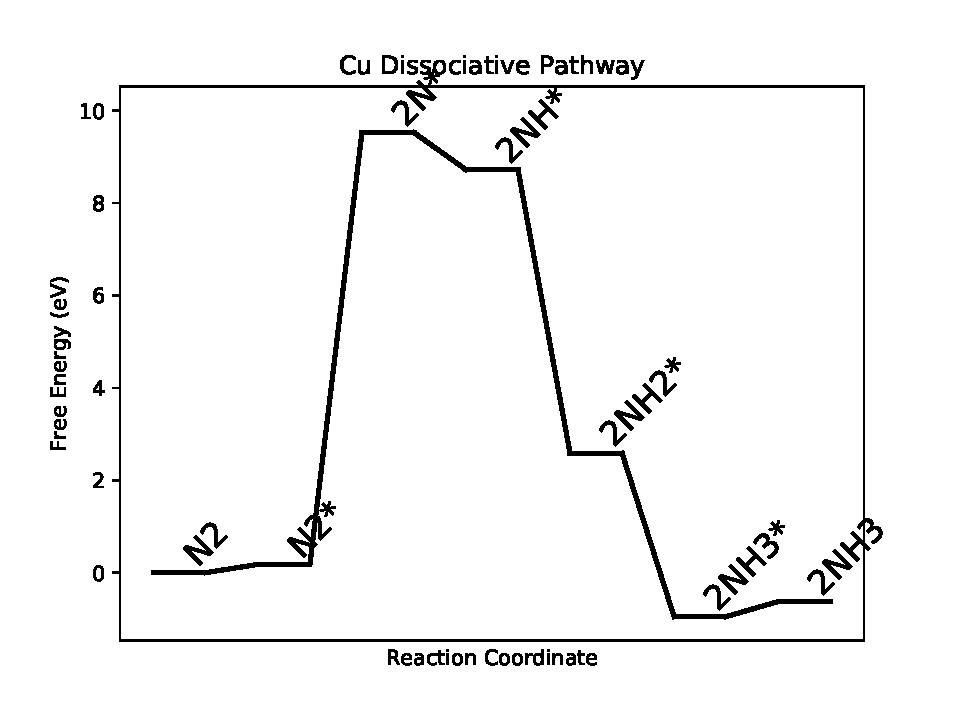
\includegraphics[width=0.8\linewidth]{data/plots/Cu_dissociative.pdf}
\end{figure}

\begin{figure}
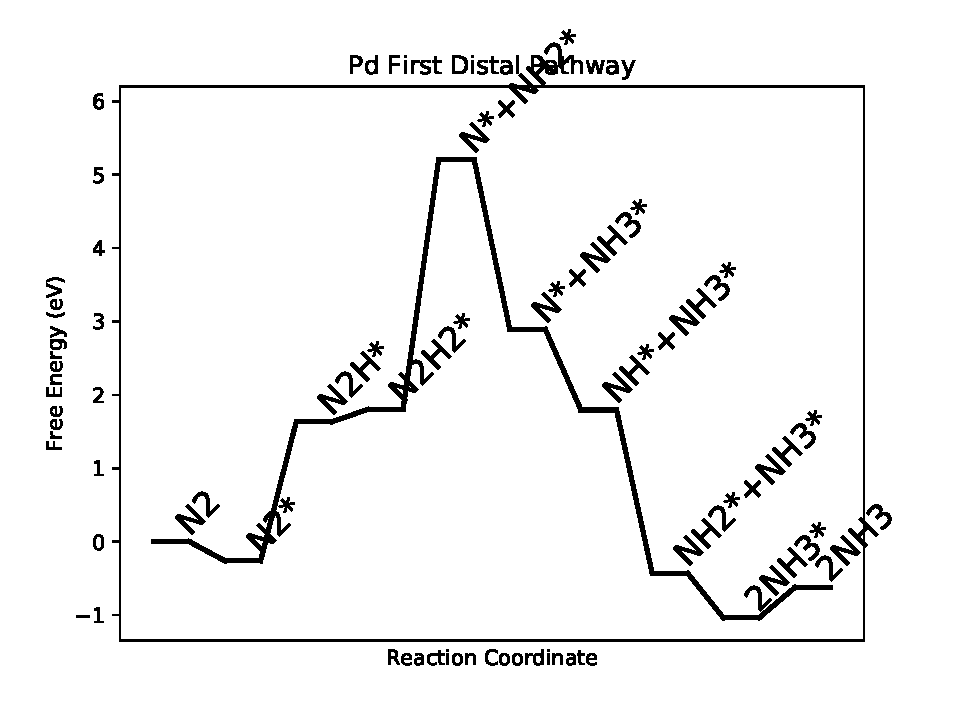
\includegraphics[width=0.8\linewidth]{data/plots/Pd_distal_1.pdf}
\end{figure}

\begin{figure}
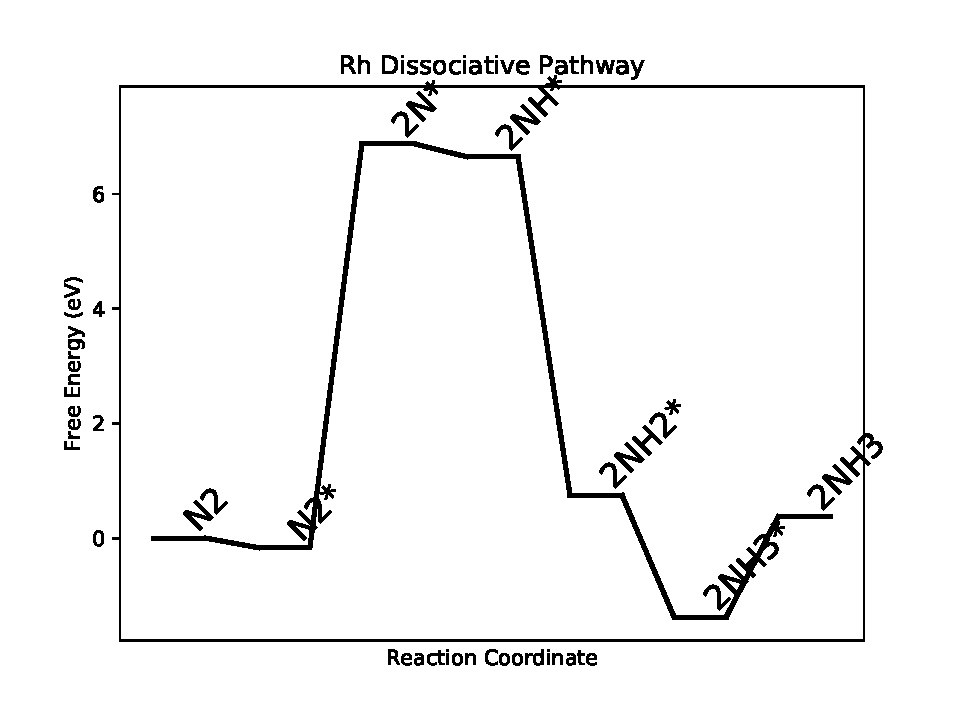
\includegraphics[width=0.8\linewidth]{data/plots/Rh_dissociative.pdf}
\end{figure}

\begin{figure}
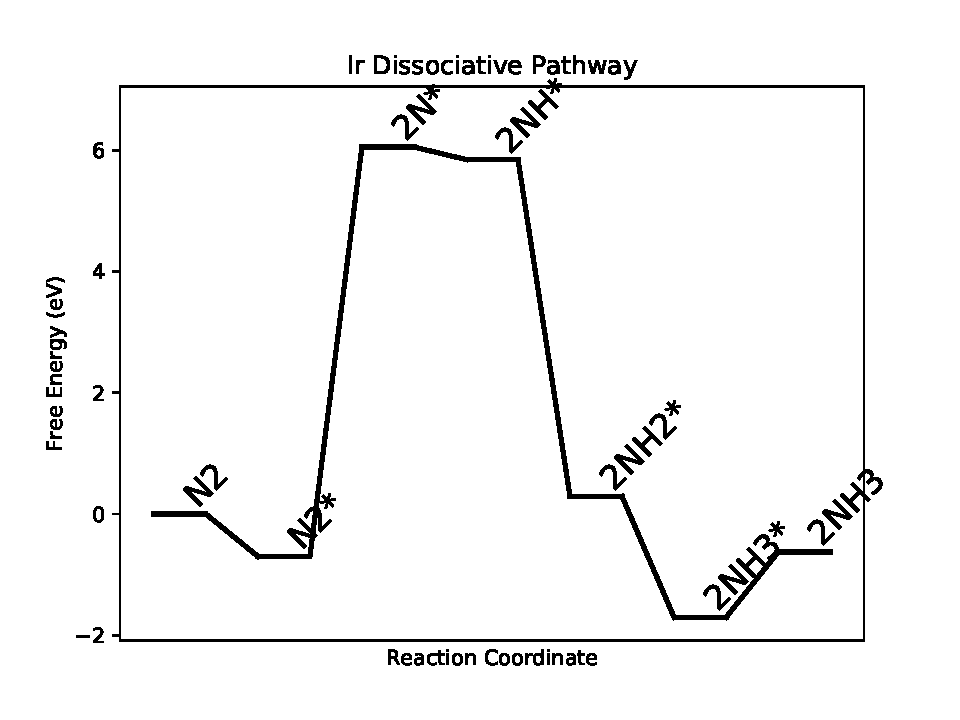
\includegraphics[width=0.8\linewidth]{data/plots/Ir_dissociative.pdf}
\end{figure}

\begin{figure}
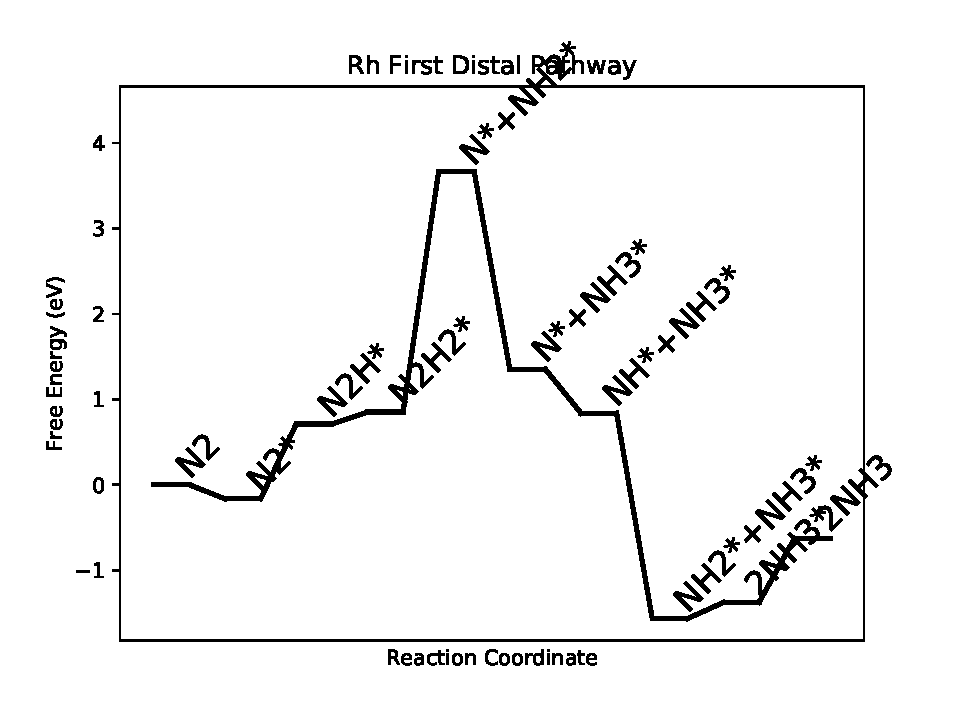
\includegraphics[width=0.8\linewidth]{data/plots/Rh_distal_1.pdf}
\end{figure}

\begin{figure}
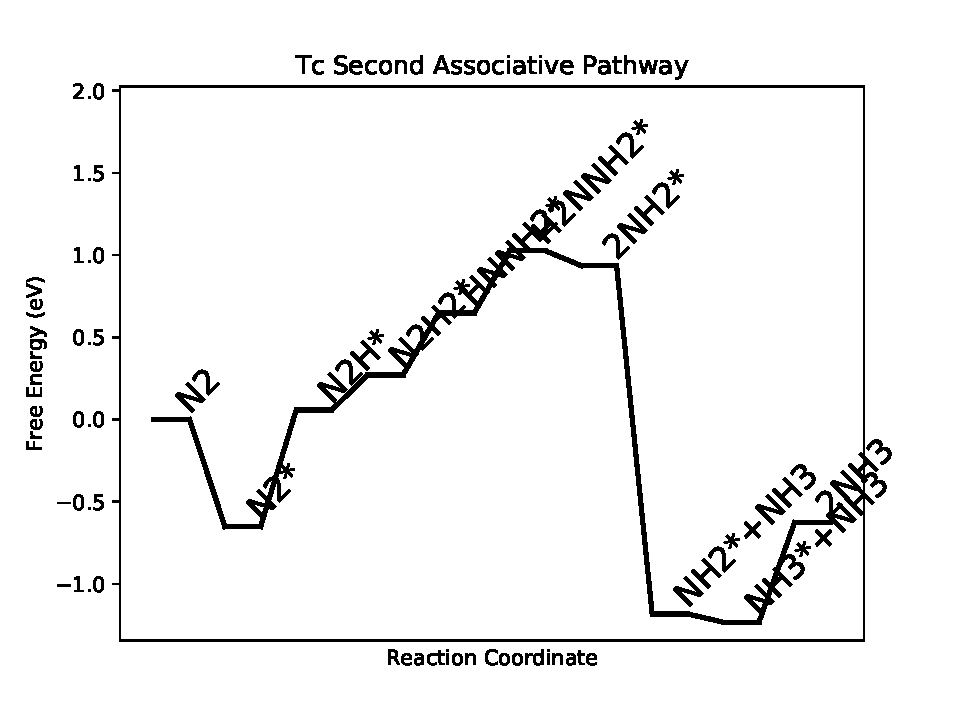
\includegraphics[width=0.8\linewidth]{data/plots/Tc_associative_2.pdf}
\end{figure}

\begin{figure}
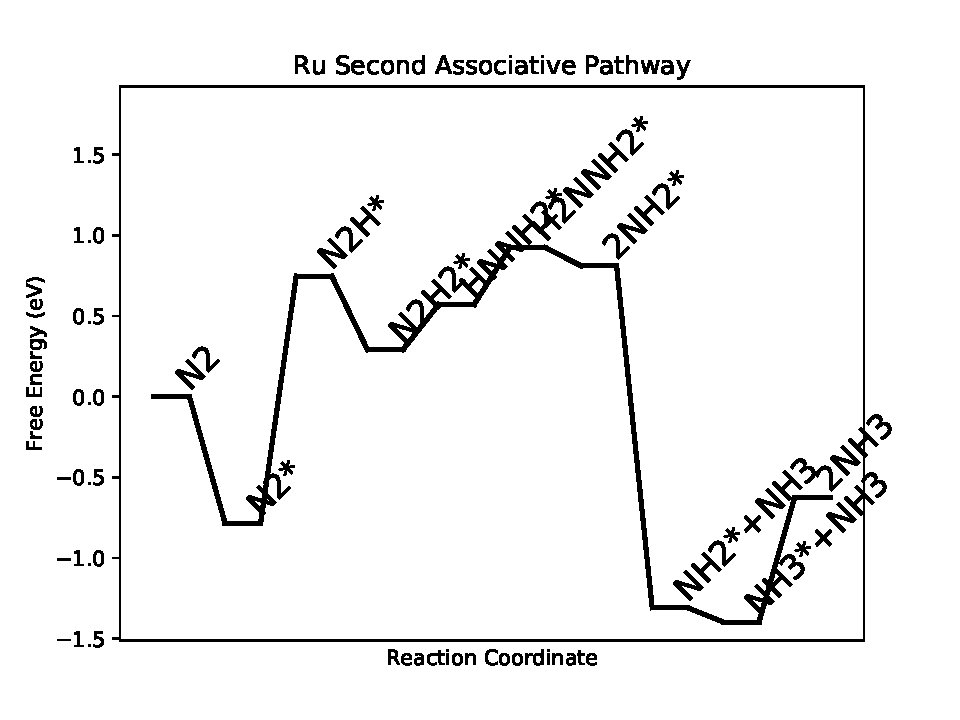
\includegraphics[width=0.8\linewidth]{data/plots/Ru_associative_2.pdf}
\end{figure}

\begin{figure}
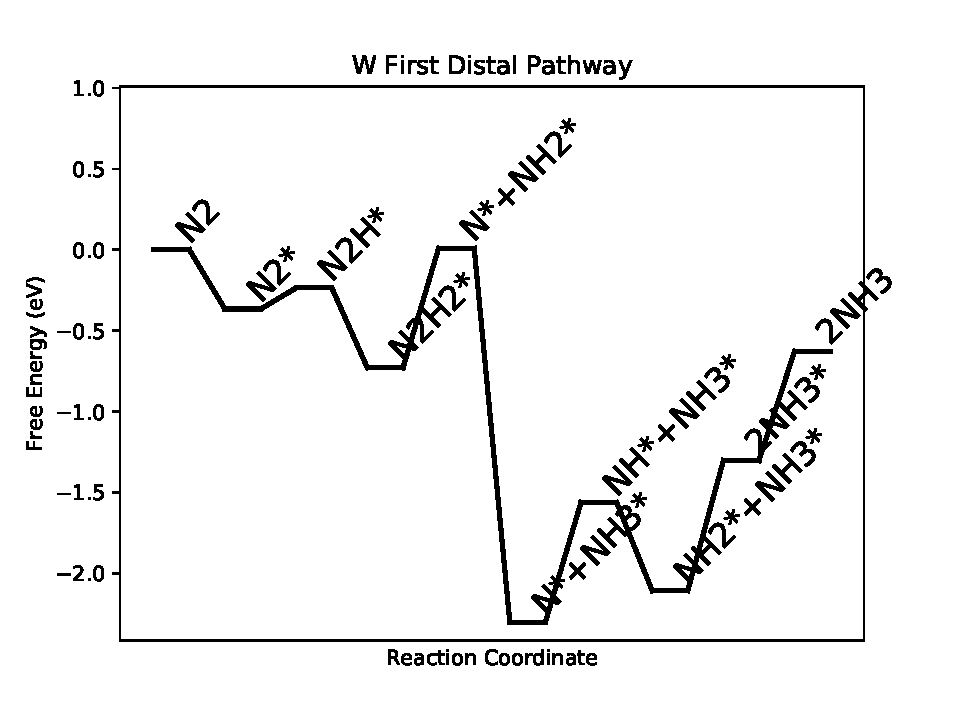
\includegraphics[width=0.8\linewidth]{data/plots/W_distal_1.pdf}
\end{figure}

\begin{figure}
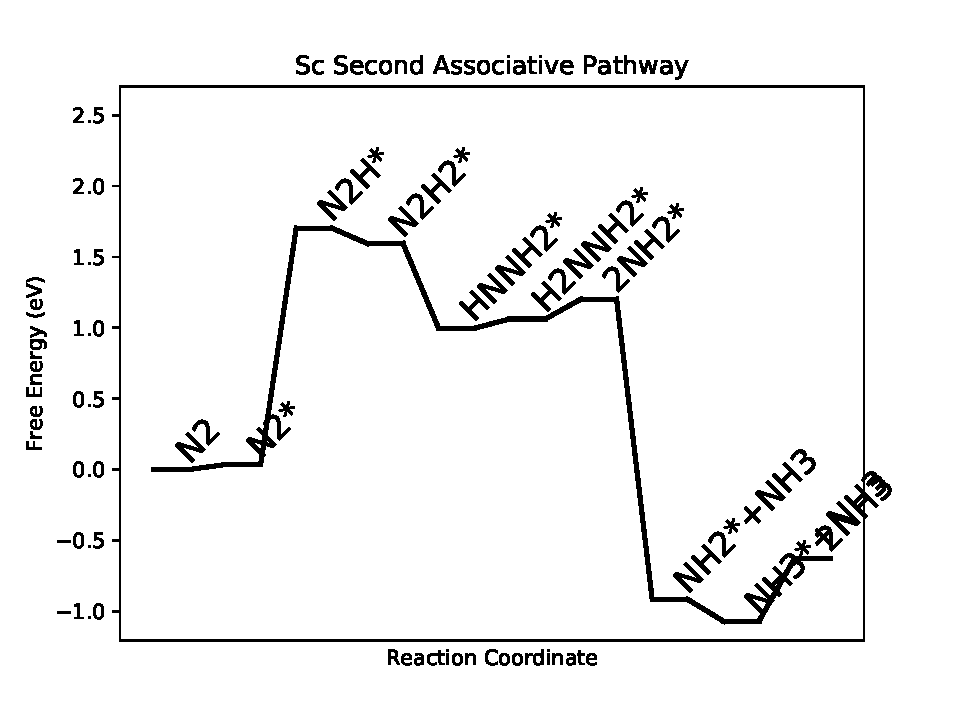
\includegraphics[width=0.8\linewidth]{data/plots/Sc_associative_2.pdf}
\end{figure}

\begin{figure}
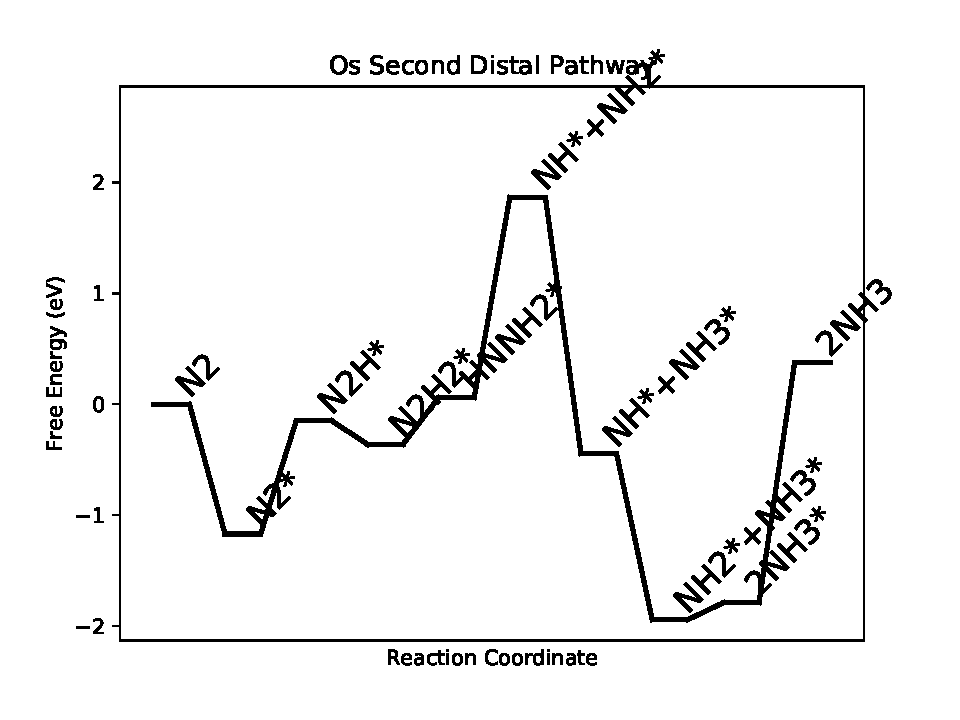
\includegraphics[width=0.8\linewidth]{data/plots/Os_distal_2.pdf}
\end{figure}

\begin{figure}
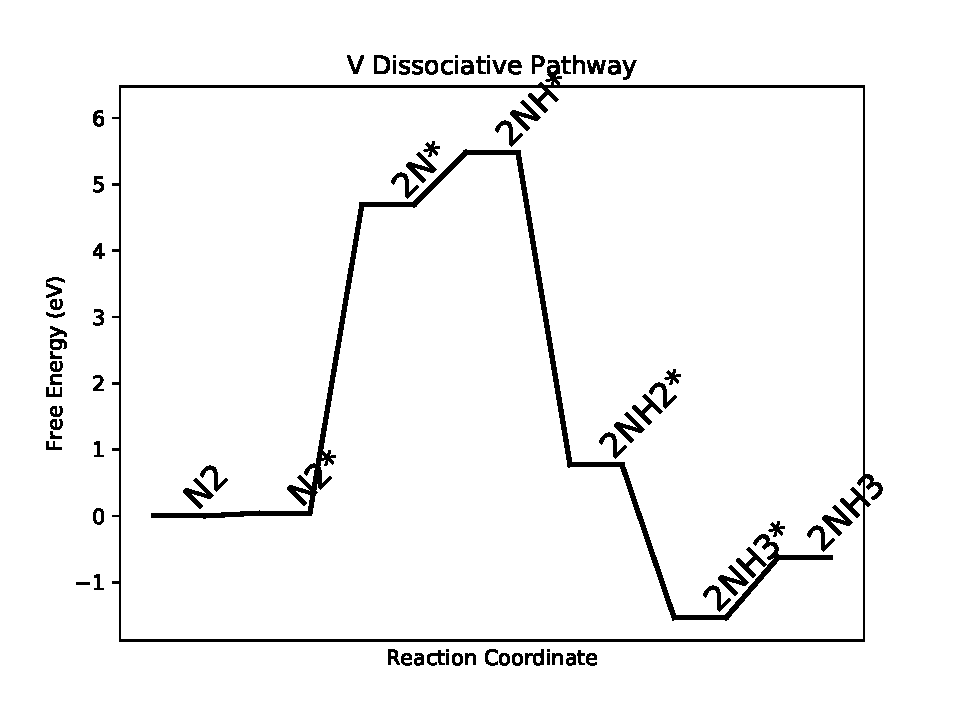
\includegraphics[width=0.8\linewidth]{data/plots/V_dissociative.pdf}
\end{figure}

\begin{figure}
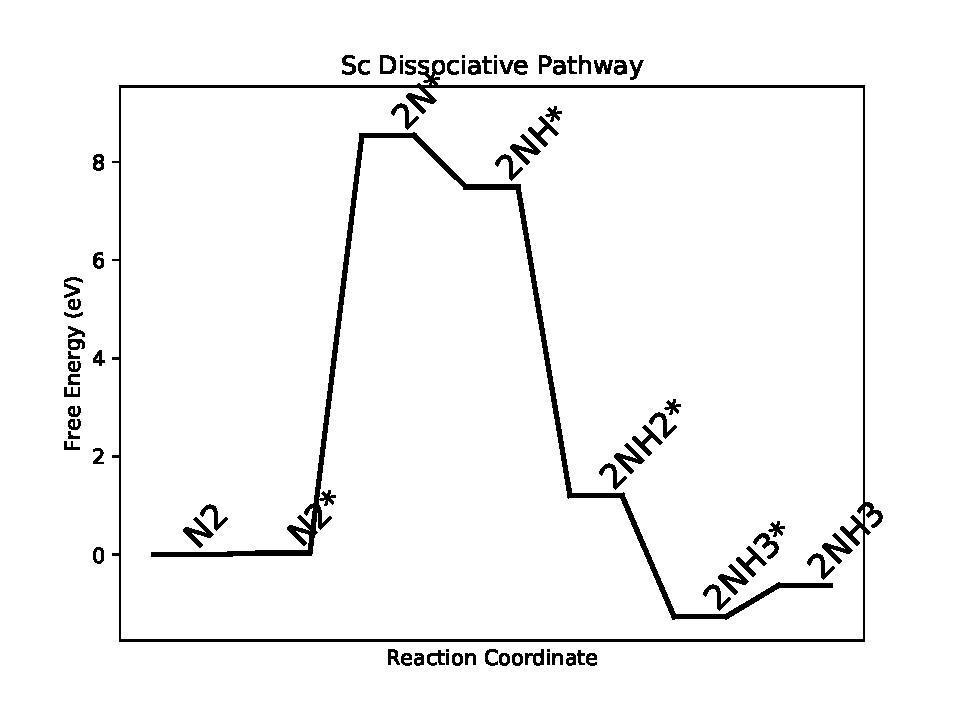
\includegraphics[width=0.8\linewidth]{data/plots/Sc_dissociative.pdf}
\end{figure}

\begin{figure}
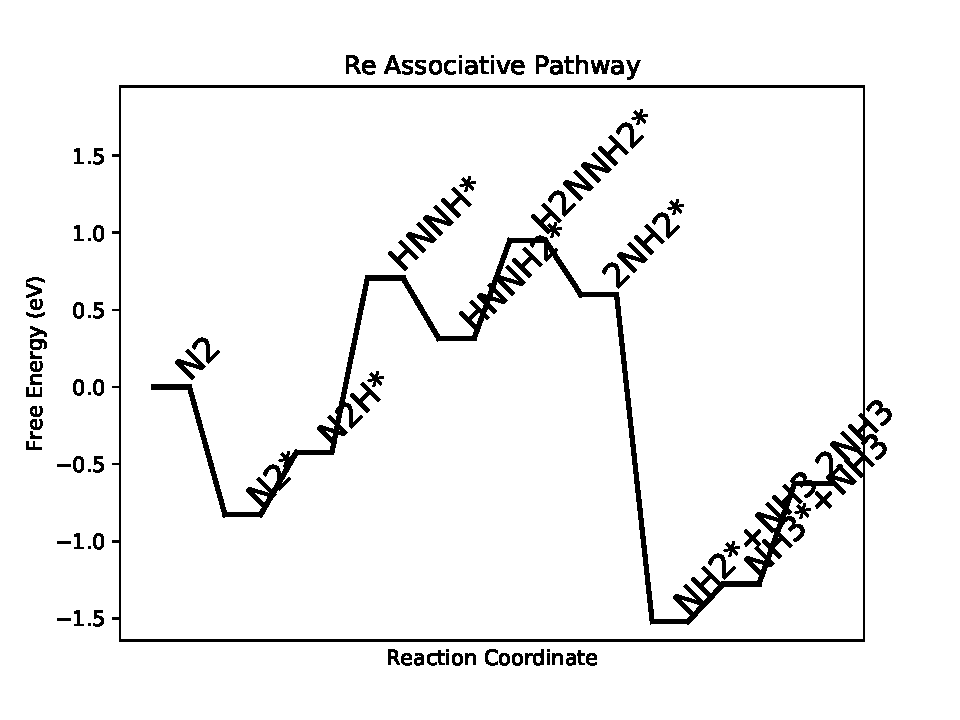
\includegraphics[width=0.8\linewidth]{data/plots/Re_associative.pdf}
\end{figure}

\begin{figure}
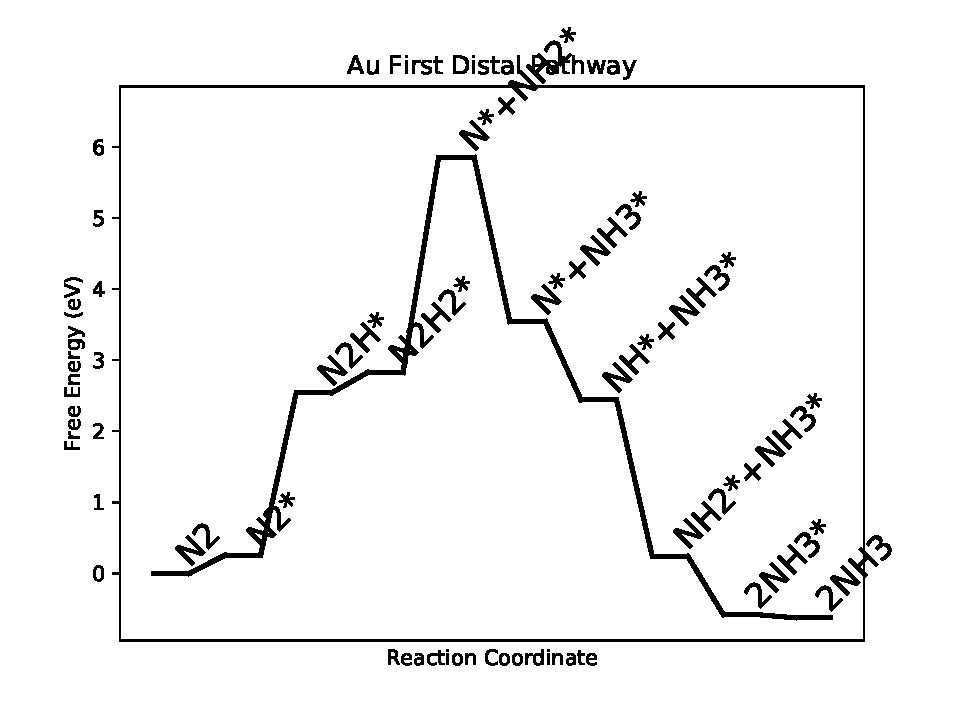
\includegraphics[width=0.8\linewidth]{data/plots/Au_distal_1.pdf}
\end{figure}

\begin{figure}
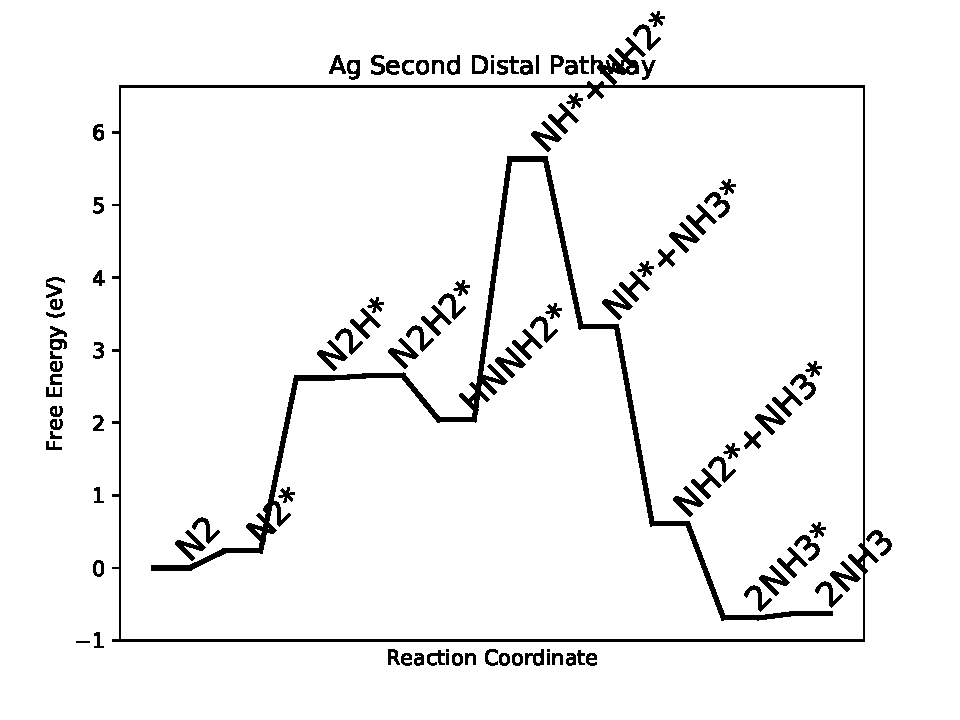
\includegraphics[width=0.8\linewidth]{data/plots/Ag_distal_2.pdf}
\end{figure}

\begin{figure}
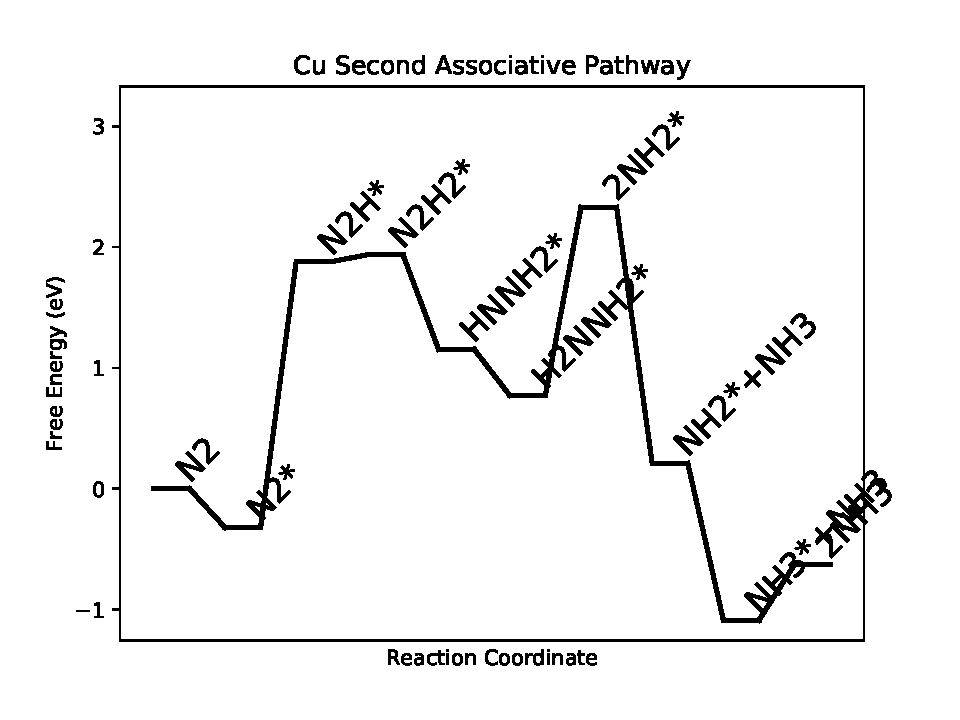
\includegraphics[width=0.8\linewidth]{data/plots/Cu_associative_2.pdf}
\end{figure}

\begin{figure}
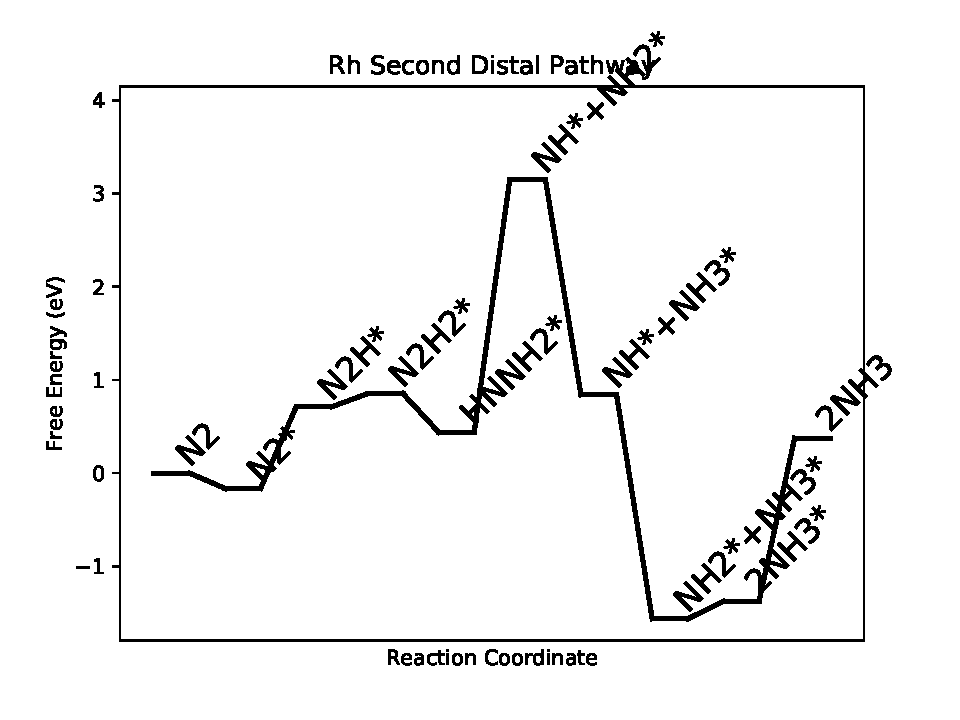
\includegraphics[width=0.8\linewidth]{data/plots/Rh_distal_2.pdf}
\end{figure}

\begin{figure}
\includegraphics[width=0.8\linewidth]{data/plots/Ir_distal_1.pdf}
\end{figure}

\begin{figure}
\includegraphics[width=0.8\linewidth]{data/plots/Cu_distal_2.pdf}
\end{figure}

\begin{figure}
\includegraphics[width=0.8\linewidth]{data/plots/Pt_distal_2.pdf}
\end{figure}

\begin{figure}
\includegraphics[width=0.8\linewidth]{data/plots/Rh_associative.pdf}
\end{figure}

\begin{figure}
\includegraphics[width=0.8\linewidth]{data/plots/Os_dissociative.pdf}
\end{figure}

\begin{figure}
\includegraphics[width=0.8\linewidth]{data/plots/Rh_associative_2.pdf}
\end{figure}

\begin{figure}
\includegraphics[width=0.8\linewidth]{data/plots/V_distal_2.pdf}
\end{figure}

\begin{figure}
\includegraphics[width=0.8\linewidth]{data/plots/Ta_distal_2.pdf}
\end{figure}

\begin{figure}
\includegraphics[width=0.8\linewidth]{data/plots/Co_distal_1.pdf}
\end{figure}

\begin{figure}
\includegraphics[width=0.8\linewidth]{data/plots/Ru_dissociative.pdf}
\end{figure}

\begin{figure}
\includegraphics[width=0.8\linewidth]{data/plots/W_dissociative.pdf}
\end{figure}

\begin{figure}
\includegraphics[width=0.8\linewidth]{data/plots/Tc_dissociative.pdf}
\end{figure}

\begin{figure}
\includegraphics[width=0.8\linewidth]{data/plots/Tc_associative.pdf}
\end{figure}

\begin{figure}
\includegraphics[width=0.8\linewidth]{data/plots/Hf_associative.pdf}
\end{figure}

\begin{figure}
\includegraphics[width=0.8\linewidth]{data/plots/Os_associative_2.pdf}
\end{figure}

\begin{figure}
\includegraphics[width=0.8\linewidth]{data/plots/Ir_associative.pdf}
\end{figure}

\begin{figure}
\includegraphics[width=0.8\linewidth]{data/plots/Cu_distal_1.pdf}
\end{figure}

\begin{figure}
\includegraphics[width=0.8\linewidth]{data/plots/Re_dissociative.pdf}
\end{figure}

\begin{figure}
\includegraphics[width=0.8\linewidth]{data/plots/Ta_associative_2.pdf}
\end{figure}

\begin{figure}
\includegraphics[width=0.8\linewidth]{data/plots/Co_associative_2.pdf}
\end{figure}

\begin{figure}
\includegraphics[width=0.8\linewidth]{data/plots/Mo_associative_2.pdf}
\end{figure}

\begin{figure}
\includegraphics[width=0.8\linewidth]{data/plots/Nb_associative.pdf}
\end{figure}

\begin{figure}
\includegraphics[width=0.8\linewidth]{data/plots/Pd_associative.pdf}
\end{figure}

\begin{figure}
\includegraphics[width=0.8\linewidth]{data/plots/Tc_distal_2.pdf}
\end{figure}

\begin{figure}
\includegraphics[width=0.8\linewidth]{data/plots/Co_dissociative.pdf}
\end{figure}

\begin{figure}
\includegraphics[width=0.8\linewidth]{data/plots/Mo_associative.pdf}
\end{figure}

\begin{figure}
\includegraphics[width=0.8\linewidth]{data/plots/Pd_distal_2.pdf}
\end{figure}

\begin{figure}
\includegraphics[width=0.8\linewidth]{data/plots/Nb_associative_2.pdf}
\end{figure}

\begin{figure}
\includegraphics[width=0.8\linewidth]{data/plots/W_associative.pdf}
\end{figure}

\begin{figure}
\includegraphics[width=0.8\linewidth]{data/plots/Ag_dissociative.pdf}
\end{figure}

\begin{figure}
\includegraphics[width=0.8\linewidth]{data/plots/Y_dissociative.pdf}
\end{figure}

\begin{figure}
\includegraphics[width=0.8\linewidth]{data/plots/Nb_dissociative.pdf}
\end{figure}

\begin{figure}
\includegraphics[width=0.8\linewidth]{data/plots/Sc_distal_1.pdf}
\end{figure}

\begin{figure}
\includegraphics[width=0.8\linewidth]{data/plots/Nb_distal_2.pdf}
\end{figure}

\begin{figure}
\includegraphics[width=0.8\linewidth]{data/plots/W_distal_2.pdf}
\end{figure}

\begin{figure}
\includegraphics[width=0.8\linewidth]{data/plots/Ta_dissociative.pdf}
\end{figure}

\begin{figure}
\includegraphics[width=0.8\linewidth]{data/plots/Tc_distal_1.pdf}
\end{figure}

\begin{figure}
\includegraphics[width=0.8\linewidth]{data/plots/Re_distal_1.pdf}
\end{figure}

\begin{figure}
\includegraphics[width=0.8\linewidth]{data/plots/Ti_associative_2.pdf}
\end{figure}

\begin{figure}
\includegraphics[width=0.8\linewidth]{data/plots/Ru_distal_1.pdf}
\end{figure}

\begin{figure}
\includegraphics[width=0.8\linewidth]{data/plots/V_associative.pdf}
\end{figure}

\begin{figure}
\includegraphics[width=0.8\linewidth]{data/plots/Ni_associative.pdf}
\end{figure}

\begin{figure}
\includegraphics[width=0.8\linewidth]{data/plots/Hf_associative_2.pdf}
\end{figure}

\begin{figure}
\includegraphics[width=0.8\linewidth]{data/plots/Re_associative_2.pdf}
\end{figure}

\begin{figure}
\includegraphics[width=0.8\linewidth]{data/plots/Ir_associative_2.pdf}
\end{figure}

\begin{figure}
\includegraphics[width=0.8\linewidth]{data/plots/Ag_associative_2.pdf}
\end{figure}

\begin{figure}
\includegraphics[width=0.8\linewidth]{data/plots/Hf_distal_2.pdf}
\end{figure}

\begin{figure}
\includegraphics[width=0.8\linewidth]{data/plots/Re_distal_2.pdf}
\end{figure}

\begin{figure}
\includegraphics[width=0.8\linewidth]{data/plots/Au_distal_2.pdf}
\end{figure}

\begin{figure}
\includegraphics[width=0.8\linewidth]{data/plots/Sc_associative.pdf}
\end{figure}

\begin{figure}
\includegraphics[width=0.8\linewidth]{data/plots/Ti_distal_2.pdf}
\end{figure}

\begin{figure}
\includegraphics[width=0.8\linewidth]{data/plots/Mo_dissociative.pdf}
\end{figure}

\begin{figure}
\includegraphics[width=0.8\linewidth]{data/plots/Zr_dissociative.pdf}
\end{figure}

\begin{figure}
\includegraphics[width=0.8\linewidth]{data/plots/Ru_associative.pdf}
\end{figure}

\begin{figure}
\includegraphics[width=0.8\linewidth]{data/plots/Ag_distal_1.pdf}
\end{figure}

\begin{figure}
\includegraphics[width=0.8\linewidth]{data/plots/Os_associative.pdf}
\end{figure}

\begin{figure}
\includegraphics[width=0.8\linewidth]{data/plots/Ag_associative.pdf}
\end{figure}

\begin{figure}
\includegraphics[width=0.8\linewidth]{data/plots/Co_distal_2.pdf}
\end{figure}

\begin{figure}
\includegraphics[width=0.8\linewidth]{data/plots/Ta_distal_1.pdf}
\end{figure}

\begin{figure}
\includegraphics[width=0.8\linewidth]{data/plots/Zr_distal_2.pdf}
\end{figure}

\begin{figure}
\includegraphics[width=0.8\linewidth]{data/plots/Ta_associative.pdf}
\end{figure}

\begin{figure}
\includegraphics[width=0.8\linewidth]{data/plots/Pt_distal_1.pdf}
\end{figure}

\begin{figure}
\includegraphics[width=0.8\linewidth]{data/plots/Cu_associative.pdf}
\end{figure}

\begin{figure}
\includegraphics[width=0.8\linewidth]{data/plots/Pd_associative_2.pdf}
\end{figure}

\begin{figure}
\includegraphics[width=0.8\linewidth]{data/plots/Pd_dissociative.pdf}
\end{figure}

\begin{figure}
\includegraphics[width=0.8\linewidth]{data/plots/Co_associative.pdf}
\end{figure}

\begin{figure}
\includegraphics[width=0.8\linewidth]{data/plots/Au_associative.pdf}
\end{figure}

\begin{figure}
\includegraphics[width=0.8\linewidth]{data/plots/V_distal_1.pdf}
\end{figure}

\begin{figure}
\includegraphics[width=0.8\linewidth]{data/plots/Ti_dissociative.pdf}
\end{figure}

\begin{figure}
\includegraphics[width=0.8\linewidth]{data/plots/Mo_distal_2.pdf}
\end{figure}

\begin{figure}
\includegraphics[width=0.8\linewidth]{data/plots/Sc_distal_2.pdf}
\end{figure}

\begin{figure}
\includegraphics[width=0.8\linewidth]{data/plots/Zr_associative_2.pdf}
\end{figure}

\begin{figure}
\includegraphics[width=0.8\linewidth]{data/plots/Zr_associative.pdf}
\end{figure}

\begin{figure}
\includegraphics[width=0.8\linewidth]{data/plots/Os_distal_1.pdf}
\end{figure}

\begin{figure}
\includegraphics[width=0.8\linewidth]{data/plots/Ti_distal_1.pdf}
\end{figure}

\begin{figure}
\includegraphics[width=0.8\linewidth]{data/plots/Hf_dissociative.pdf}
\end{figure}

\begin{figure}
\includegraphics[width=0.8\linewidth]{data/plots/W_associative_2.pdf}
\end{figure}

\begin{figure}
\includegraphics[width=0.8\linewidth]{data/plots/Zr_distal_1.pdf}
\end{figure}

\begin{figure}
\includegraphics[width=0.8\linewidth]{data/plots/Hf_distal_1.pdf}
\end{figure}


\end{document}
One route to increasing reaction rates is the the inclusion of transition-metal dopants in TiO$_2$. Transition-metal dopants can increase rates via two distinct mechanisms: increasing the amount of photo-generated electrons that reach the surface by improving absorption and charge separation, or by altering the kinetics of the surface reaction.

